% =============================================================================
% AIGGPA Bhopal — Internship Pre-Joining Research Report
% HR–IT Integration in Govt Sector & Technology Assessment of Officials
% Compiled: April 2026 | Secondary Research (Desk Study)
% =============================================================================
\documentclass[12pt,a4paper]{article}

%  --  Packages  -- 
\usepackage{fontspec}
\setmainfont{Latin Modern Roman}
\newfontfamily{\hindifont}{Nirmala UI}[Script=Devanagari]
\newcommand{\hindi}[1]{{\hindifont #1}}
\newcommand{\INR}{{\hindifont ₹}}
\usepackage[margin=2.5cm]{geometry}
\usepackage{graphicx}
\usepackage{xcolor}
\usepackage{booktabs}
\usepackage{tabularx}
\usepackage{longtable}
\usepackage{multirow}
\usepackage{enumitem}
\usepackage{tikz}
\usepackage{pgfplots}
\usepackage{pgfplotstable}
\usepackage{float}
\usepackage{caption}
\usepackage{subcaption}
\usepackage{hyperref}
\usepackage{fancyhdr}
\usepackage{titlesec}
\usepackage{setspace}
\usepackage{tcolorbox}
\usepackage{amssymb}
\usepackage{pifont}
\usepackage{array}

\pgfplotsset{compat=1.18}
\usetikzlibrary{shapes.geometric, arrows.meta, positioning, calc, patterns, shadows, decorations.markings}

%  --  Colour Palette  -- 
\definecolor{govblue}{HTML}{1B3B6F}
\definecolor{govgold}{HTML}{FFC107}
\definecolor{govred}{HTML}{B22234}
\definecolor{accent1}{HTML}{1B4F72}
\definecolor{accent2}{HTML}{2E86C1}
\definecolor{accent3}{HTML}{27AE60}
\definecolor{accent4}{HTML}{E67E22}
\definecolor{accent5}{HTML}{8E44AD}
\definecolor{lightgray}{HTML}{F2F3F4}
\definecolor{boxbg}{HTML}{EBF5FB}
\definecolor{warningbg}{HTML}{FFF3CD}
\definecolor{successbg}{HTML}{D4EDDA}

%  --  tcolorbox styles  -- 
\tcbuselibrary{skins, breakable}

\newtcolorbox{sourcebox}[1][]{
  colback=boxbg, colframe=accent2, 
  fonttitle=\bfseries, title={#1},
  boxrule=0.5pt, arc=2mm, breakable
}

\newtcolorbox{warningbox}[1][]{
  colback=warningbg, colframe=accent4,
  fonttitle=\bfseries, title={#1},
  boxrule=0.5pt, arc=2mm
}

\newtcolorbox{notebox}[1][]{
  colback=successbg, colframe=accent3,
  fonttitle=\bfseries, title={#1},
  boxrule=0.5pt, arc=2mm
}

%  --  Header/Footer  -- 
\pagestyle{fancy}
\fancyhf{}
\fancyhead[L]{\small\textcolor{govblue}{AIGGPA Bhopal  --  Internship Research Report}}
\fancyhead[R]{\small\textcolor{govblue}{April 2026}}
\fancyfoot[C]{\thepage}
\renewcommand{\headrulewidth}{0.4pt}

%  --  Section Formatting  -- 
\titleformat{\section}
  {\Large\bfseries\color{govblue}}{\thesection}{1em}{}[\titlerule]
\titleformat{\subsection}
  {\large\bfseries\color{accent1}}{\thesubsection}{1em}{}
\titleformat{\subsubsection}
  {\normalsize\bfseries\color{accent2}}{\thesubsubsection}{1em}{}

%  --  Spacing  -- 
\setstretch{1.25}

%  --  Hyperref  -- 
\hypersetup{
  colorlinks=true, linkcolor=govblue, urlcolor=accent2, citecolor=accent5
}

% =============================================================================
\begin{document}

%  --  Title Page  -- 
\begin{titlepage}
\begin{center}

\vspace*{1cm}

%  --  Ashoka Chakra / Emblem placeholder via TikZ  -- 

\begin{tikzpicture}
  \draw[govblue, line width=2pt] (0,0) circle (1.5cm);
  \foreach \i in {0,15,...,345} {
    \draw[govblue, line width=0.8pt] (0,0) -- (\i:1.4cm);
  }
  \draw[govblue, line width=1.5pt] (0,0) circle (0.35cm);
  \draw[govblue, line width=1.5pt] (0,0) circle (1.0cm);
\end{tikzpicture}

\vspace{1cm}

{\Huge\bfseries\textcolor{govblue}{HR--IT Integration in the}\\\textcolor{govblue}{Government Sector}}

{\large\textcolor{accent1}{\hindi{शासकीय क्षेत्र में मानव संसाधन-सूचना प्रौद्योगिकी एकीकरण}}}

\vspace{0.5cm}

{\LARGE\textcolor{accent1}{\&}}

\vspace{0.5cm}

{\Huge\bfseries\textcolor{govblue}{Technology Assessment of}\\\textcolor{govblue}{Class~I, II \& III Officials}}

{\large\textcolor{accent1}{\hindi{वर्ग I, II एवं III अधिकारियों का प्रौद्योगिकी मूल्यांकन}}}

\vspace{1.5cm}

\rule{0.6\textwidth}{1pt}

\vspace{0.5cm}

{\Large Secondary Research Report (Desk Study)}

\vspace{0.5cm}

{\large Prepared for the Summer Internship at}

\vspace{0.3cm}

{\Large\bfseries\textcolor{govgold}{Atal Bihari Vajpayee Institute of\\Good Governance \& Policy Analysis}}

{\large\textcolor{govgold}{\hindi{अटल बिहारी वाजपेयी सुशासन एवं नीति विश्लेषण संस्थान}}}

{\large\textcolor{govgold}{(AIGGPA), Bhopal, Madhya Pradesh / \hindi{भोपाल, मध्य प्रदेश}}}

\vspace{1cm}

\rule{0.6\textwidth}{1pt}

\vspace{0.8cm}

{\large\textbf{Date:} April 2026}

\vspace{0.3cm}

{\large\textbf{Duration:} 3-Month Summer Internship}

\vspace{0.3cm}

{\large\textbf{Methodology:} Secondary Sources  --  Government Publications,\\Policy Documents, Official Platform Data, Academic Research}

\vfill

{\small\textcolor{gray}{This document contains only verified data from official government sources (PIB, DARPG, DoPT, NIC, GeM, MeitY).\\All figures are cited with source attributions. Estimates are clearly marked as such.}}

\end{center}
\end{titlepage}

%  --  Table of Contents  -- 
\tableofcontents
\newpage

% =============================================================================
% PART I
% =============================================================================
\part{HR--IT Integration in the Government Sector}
\begin{center}{\Large\hindi{भाग 1: शासकीय क्षेत्र में मानव संसाधन-सूचना प्रौद्योगिकी एकीकरण}}\end{center}

\section{Introduction \& Context}

\subsection{The Scale of India's Government Workforce (\hindi{भारत सरकार का कार्यबल})}

The Government of India is one of the largest employers in the world. Managing this vast, geographically dispersed workforce through traditional paper-based systems has been a persistent bottleneck in governance efficiency.

\begin{table}[H]
\centering
\caption{Central Government Employee Strength}
\label{tab:workforce}
\begin{tabular}{@{}lrl@{}}
\toprule
\textbf{Parameter} & \textbf{Figure} & \textbf{Source} \\
\midrule
Central Govt Civilian Employees (est.\ 2024) & 35.1 lakh & Budget Documents / Indiastat \\
Sanctioned posts remaining vacant & 9--10 lakh & DoPT Annual Report \\
\bottomrule
\end{tabular}
\end{table}

\begin{warningbox}[Note on State Government Data]
There is no single centralised national database aggregating total state government employees. Each of India's 36 States and UTs maintains its own HR and payroll data independently. Therefore, precise nationwide aggregate figures for state employees are not publicly available.
\end{warningbox}

\subsection{What is HR--IT Integration? (\hindi{मानव संसाधन-सूचना प्रौद्योगिकी एकीकरण क्या है?})}

\textbf{HR--IT Integration} refers to the convergence of Human Resource Management functions with Information Technology systems to create unified, digital, data-driven workforce management platforms. In the government sector, this is not merely an efficiency exercise -- it is a \textbf{governance reform imperative} that directly impacts transparency, accountability, and citizen service delivery.

\begin{table}[H]
\centering
\caption{Traditional vs.\ Digitally Integrated HR Processes}
\label{tab:tradvsdigital}
\begin{tabularx}{\textwidth}{@{}lXX@{}}
\toprule
\textbf{Dimension} & \textbf{Traditional (Pre-Digital)} & \textbf{Integrated (Post-Digital)} \\
\midrule
Service Records & Physical files, prone to loss & Digital e-Service Books, 24/7 access \\
Leave/Claims & Multi-step paper forms, weeks long & Self-service portals, real-time tracking \\
Transfers/Postings & Opaque, manual, prone to manipulation & Rule-based, transparent, algorithmic \\
Performance Appraisal & Paper ACRs, delayed, subjective & SPARROW e-APAR, time-bound, digital \\
Training & Ad-hoc, seniority-based & Competency-mapped (iGOT), role-based \\
Decision Support & Intuition-based & Data analytics, dashboards, AI-enabled \\
\bottomrule
\end{tabularx}
\end{table}

% =============================================================================
\section{Key Digital Platforms Powering HR--IT Integration}

\subsection{e-HRMS (Electronic Human Resource Management System)}
\noindent\hindi{इलेक्ट्रॉनिक मानव संसाधन प्रबंधन प्रणाली} \\[0.3em]

\begin{sourcebox}[Platform Overview]
\begin{tabularx}{\textwidth}{@{}lX@{}}
\textbf{Developer:} & National Informatics Centre (NIC) \\
\textbf{Custodian:} & Department of Personnel \& Training (DoPT), Government of India \\
\textbf{Launch:} & e-HRMS 1.0 in 2017; \textbf{e-HRMS 2.0} in December 2022 \\
\textbf{Scope:} & All Central Government employees \\
\textbf{Access:} & Via NIC's unified SSO platform  --  \textbf{Parichay} \\
\textbf{Sources:} & PIB, Informatics (NIC journal), HRMSpedia \\
\end{tabularx}
\end{sourcebox}

\subsubsection{Core Modules}

\begin{enumerate}[label=\arabic*., leftmargin=2cm]
  \item \textbf{Personnel Information System (PIS)}  --  comprehensive employee database
  \item \textbf{Leave Management}  --  online applications, auto-routing, balance tracking
  \item \textbf{LTC (Leave Travel Concession)}  --  digital claims and settlement
  \item \textbf{Loans \& Advances}  --  application, approval, disbursement tracking
  \item \textbf{Tours \& Reimbursements}  --  end-to-end digital workflow
  \item \textbf{Salary \& GPF Details}  --  integrated with payroll systems
  \item \textbf{e-Service Book}  --  digitised service records with automated updates
\end{enumerate}

\subsubsection{Strategic Capabilities}
\begin{itemize}
  \item \textbf{Employee Self-Service (ESS):} View/update personal data, apply for services, track approvals via web or mobile app (e-HRMS 2.0)
  \item \textbf{Dashboard Analytics:} Real-time dashboards for senior authorities showing pendency, data update status, and HR analytics
  \item \textbf{Integration:} Linked with APAR (Annual Performance Assessment Report) and iGOT Karmayogi training records
  \item \textbf{``Right Person for the Right Post'':} Matching qualifications and experience to vacancies for data-driven postings
\end{itemize}

%  -- 
\subsection{e-Office (\hindi{ई-कार्यालय})}

\begin{sourcebox}[Platform Overview]
\begin{tabularx}{\textwidth}{@{}lX@{}}
\textbf{Purpose:} & Paperless office operations  --  eFile, eReceipt \\
\textbf{Standards:} & Based on Central Secretariat Manual of Office Procedure (CSMOP) \\
\textbf{Manager:} & DARPG with NIC technical support \\
\textbf{Sources:} & PIB, Economic Times, DARPG official releases \\
\end{tabularx}
\end{sourcebox}

\subsubsection{Verified Statistics}

\begin{table}[H]
\centering
\caption{e-Office Adoption  --  Verified Data Points}
\label{tab:eoffice}
\begin{tabular}{@{}p{7cm}rl@{}}
\toprule
\textbf{Metric} & \textbf{Value} & \textbf{Source} \\
\midrule
Files handled as e-files (cumulative) & 37+ lakh & PIB, Oct 2024 \\
Electronic file processing (Central Sectt.) & 94\% & PIB / ET, mid-2024 \\
Electronic receipt processing (Central Sectt.) & 95\% & PIB / ET, mid-2024 \\
Ministries/Departments using e-Office & 74 & PIB \\
Active users & 47,000+ & PIB \\
Total organisations onboarded & 393 & PIB, late 2024 \\
Orgs onboarded under 100-day agenda & 92 of 133 & PIB, Oct 2024 \\
Users covered in 100-day expansion & 6,500 & PIB \\
Migration to eOffice 7.0 began & Feb 2023 & Economic Times \\
Ministries migrated to eOffice 7.0 & 58 & ET \\
Departments migrated to eOffice 7.0 & 98 & ET \\
\bottomrule
\end{tabular}
\end{table}

%  --  e-Office Growth Chart  -- 
\begin{figure}[H]
\centering
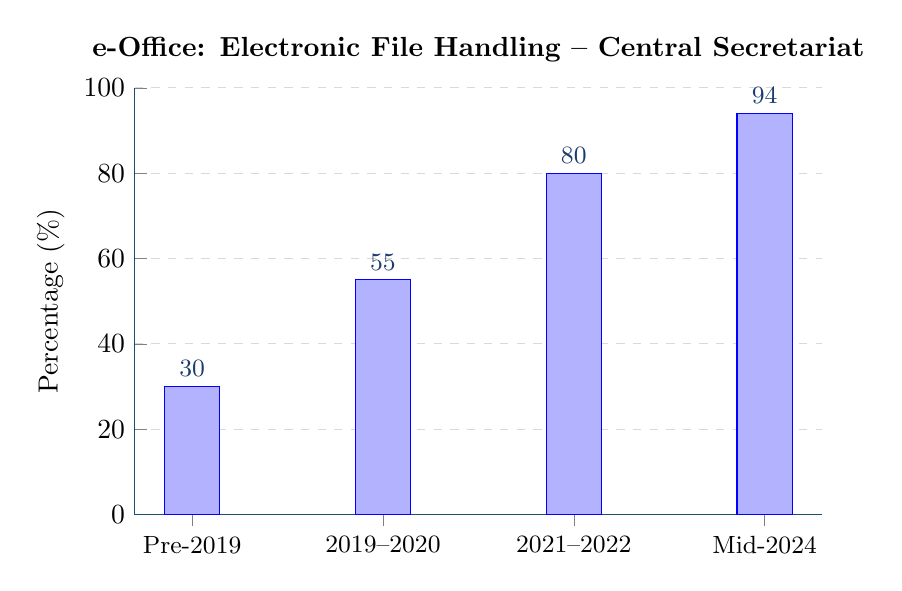
\begin{tikzpicture}
\begin{axis}[
    title={\textbf{e-Office: Electronic File Handling  --  Central Secretariat}},
    width=0.85\textwidth,
    height=7cm,
    ybar,
    bar width=20pt,
    ylabel={Percentage (\%)},
    symbolic x coords={Pre-2019, 2019--2020, 2021--2022, Mid-2024},
    xtick=data,
    ymin=0, ymax=100,
    nodes near coords,
    nodes near coords align={vertical},
    every node near coord/.append style={font=\small\bfseries, color=govblue},
    fill=accent2!80,
    draw=accent1,
    axis lines*=left,
    ymajorgrids=true,
    grid style={dashed, gray!30},
    x tick label style={font=\small, align=center},
    legend style={at={(0.5,-0.2)}, anchor=north, font=\footnotesize},
]
\addplot coordinates {(Pre-2019, 30) (2019--2020, 55) (2021--2022, 80) (Mid-2024, 94)};
\end{axis}
\end{tikzpicture}
\caption{Growth of electronic file processing in the Central Secretariat. Pre-2019 and 2019--2020 figures are approximate based on DARPG reports describing ``majority still paper-based'' and ``COVID-accelerated adoption.'' The 2021--22 figure reflects post-pandemic acceleration. Mid-2024 figure (94\%) is directly from PIB.}
\label{fig:eoffice_growth}
\end{figure}

%  -- 
\subsection{iGOT Karmayogi (Mission Karmayogi / \hindi{मिशन कर्मयोगी})}

\begin{sourcebox}[Platform Overview]
\begin{tabularx}{\textwidth}{@{}lX@{}}
\textbf{Full Name:} & Integrated Government Online Training  --  Mission Karmayogi \\
\textbf{Launch:} & 2020 (National Programme for Civil Services Capacity Building) \\
\textbf{Framework:} & Karmayogi Competency Model (KCM)  --  Attitude, Skills, Knowledge (ASK) \\
\textbf{Paradigm Shift:} & From rule-based $\rightarrow$ \textbf{role-based} training \\
\textbf{Sources:} & PIB (multiple releases), DD News, iGOT portal, Drishti IAS \\
\end{tabularx}
\end{sourcebox}

\subsubsection{Verified Growth Statistics}

\begin{table}[H]
\centering
\caption{iGOT Karmayogi  --  Verified Milestones}
\label{tab:igot}
\begin{tabular}{@{}p{6.5cm}rl@{}}
\toprule
\textbf{Metric} & \textbf{Value} & \textbf{Source / Date} \\
\midrule
Registered users (Jan 2023) & $\sim$3 lakh & PIB \\
Registered users (May 2025) & 1 crore+ & PIB, 21 May 2025 \\
Registered users (Jul 2025) & 1.26 crore & PIB, 21 Jul 2025 \\
Registered users (Mar 2026) & 1.53 crore+ & PIB, 27 Mar 2026 \\
Central govt users (Jul 2025) & $\sim$41 lakh & DD India \\
State/UT users (Jul 2025) & $\sim$85 lakh & DD India \\
Live courses & 4,600+ & PIB, Mar 2026 \\
Languages supported & 16 & PIB \\
Course completions (cumulative) & 8.3 crore+ & PIB, Mar 2026 \\
Learning certificates issued & 3.1 crore+ & Drishti IAS / PIB \\
Cumulative learning hours & 3.8 crore+ & PIB \\
AI-related course learners & 1.3 million+ & IndiaAI.gov.in \\
Contributing partners & 200+ & PIB \\
Karmayogi Saptah completions (Oct 2024) & 32 lakh & PIB / DD News \\
Karmayogi Saptah learning hours (Oct 2024) & 38 lakh & PIB / DD News \\
Jan Seva Programme trained (Jan 2025) & 8.5 lakh & PIB \\
\bottomrule
\end{tabular}
\end{table}

%  --  iGOT Growth Chart  -- 
\begin{figure}[H]
\centering
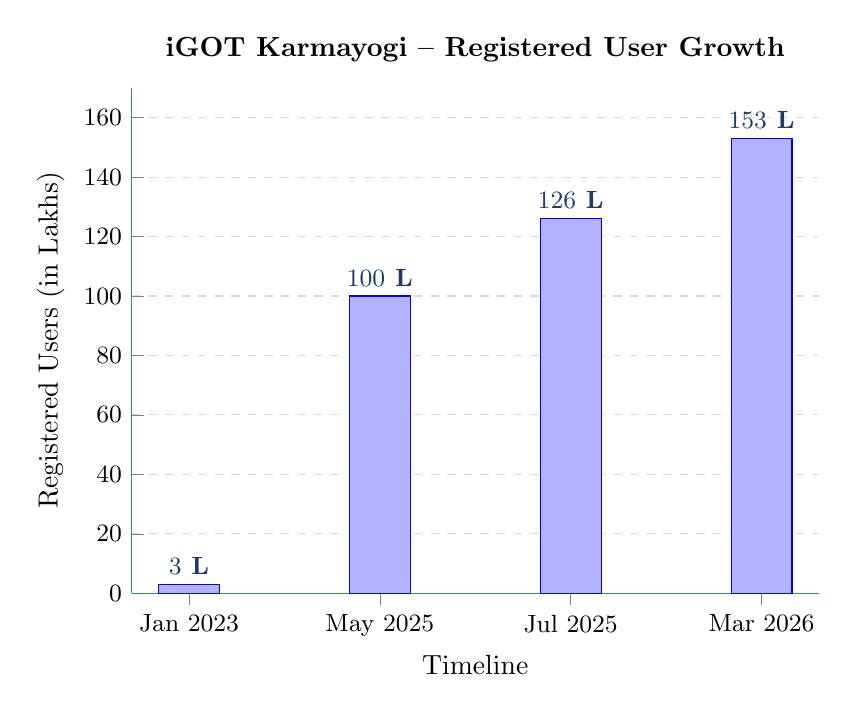
\begin{tikzpicture}
\begin{axis}[
    title={\textbf{iGOT Karmayogi  --  Registered User Growth}},
    width=0.85\textwidth,
    height=8cm,
    xlabel={Timeline},
    ylabel={Registered Users (in Lakhs)},
    symbolic x coords={Jan 2023, May 2025, Jul 2025, Mar 2026},
    xtick=data,
    ymin=0, ymax=170,
    nodes near coords={\pgfmathprintnumber{\pgfplotspointmeta} L},
    nodes near coords align={vertical},
    every node near coord/.append style={font=\small\bfseries, color=govblue},
    ybar,
    bar width=22pt,
    fill=accent3!75,
    draw=accent3!90!black,
    axis lines*=left,
    ymajorgrids=true,
    grid style={dashed, gray!30},
    x tick label style={font=\small},
    y tick label style={font=\small},
    area legend,
]
\addplot coordinates {(Jan 2023, 3) (May 2025, 100) (Jul 2025, 126) (Mar 2026, 153)};
\end{axis}
\end{tikzpicture}
\caption{iGOT Karmayogi registered user growth from January 2023 to March 2026 (30$\times$ growth in $\sim$28 months). All figures from PIB official press releases.}
\label{fig:igot_growth}
\end{figure}

%  --  iGOT User Composition Pie Chart  -- 
\begin{figure}[H]
\centering
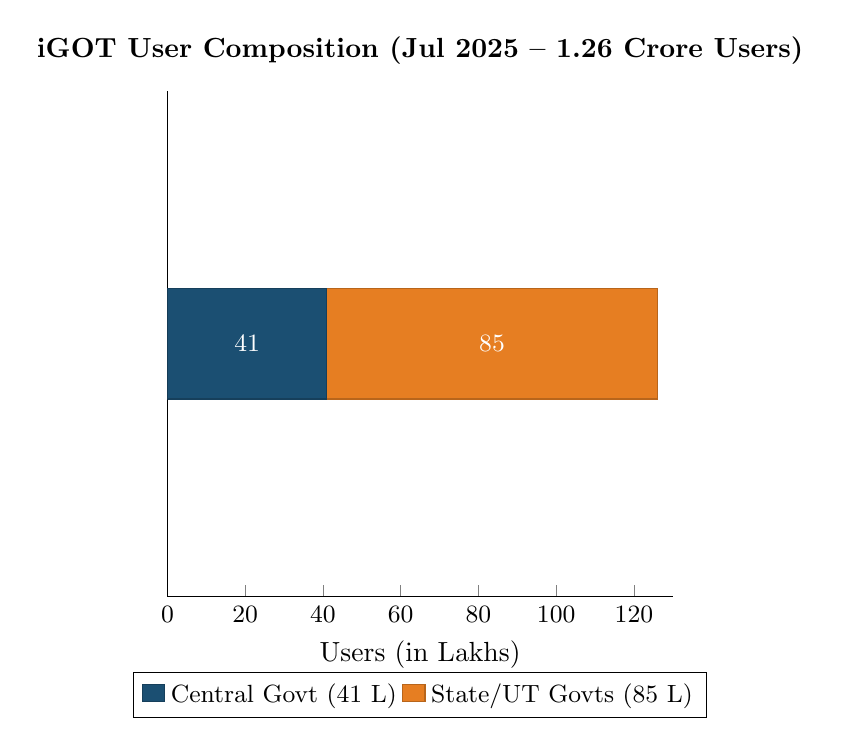
\begin{tikzpicture}
\begin{axis}[
    title={\textbf{iGOT User Composition (Jul 2025  --  1.26 Crore Users)}},
    width=8cm, height=8cm,
    xbar stacked,
    xmin=0, xmax=130,
    ytick={1},
    yticklabels={},
    bar width=40pt,
    xlabel={Users (in Lakhs)},
    legend style={at={(0.5,-0.15)}, anchor=north, legend columns=2, font=\small},
    axis lines*=left,
    x tick label style={font=\small},
    nodes near coords,
    every node near coord/.append style={font=\small\bfseries, color=white, anchor=center},
]
\addplot[fill=accent1, draw=accent1!80!black] coordinates {(41,1)};
\addplot[fill=accent4, draw=accent4!80!black] coordinates {(85,1)};
\legend{Central Govt (41 L), State/UT Govts (85 L)}
\end{axis}
\end{tikzpicture}
\caption{Composition of iGOT Karmayogi users: Central vs.\ State/UT government employees. Source: DD India, July 2025.}
\label{fig:igot_composition}
\end{figure}

%  -- 
\subsection{Other Key Platforms in the HR--IT Ecosystem}

\begin{table}[H]
\centering
\caption{Digital Platforms Used by Government Officials}
\label{tab:platforms}
\begin{tabularx}{\textwidth}{@{}lXl@{}}
\toprule
\textbf{Platform} & \textbf{Function} & \textbf{Source} \\
\midrule
SPARROW & Electronic Performance Appraisal Reports (APARs), replacing paper ACRs & DARPG/NIC \\
PFMS & End-to-end fund tracking, payroll, DBT disbursement & CGA, MoF \\
GeM & Government e-Marketplace for digital procurement & MoCI / GeM \\
CPGRAMS & AI/ML-powered citizen grievance redressal & DARPG \\
GEMS & Govt Employees Management System (HR records, payroll, MIS) & DoPT \\
Parichay & NIC unified SSO for all government applications & NIC \\
AEBAS & Aadhaar-Enabled Biometric Attendance System & DoPT \\
\bottomrule
\end{tabularx}
\end{table}

%  --  GeM Growth Chart  -- 
\begin{figure}[H]
\centering
\begin{tikzpicture}
\begin{axis}[
    title={\textbf{GeM  --  Gross Merchandise Value Growth (\INR\ Crore)}},
    width=0.9\textwidth,
    height=8cm,
    xlabel={Financial Year},
    ylabel={GMV (Rs.\ Crore)},
    symbolic x coords={FY17, FY18, FY19, FY20, FY21, FY22, FY23, FY24, FY25},
    xtick=data,
    ymin=0, ymax=600000,
    ybar,
    bar width=14pt,
    fill=govgold!80,
    draw=govgold!90!black,
    axis lines*=left,
    ymajorgrids=true,
    grid style={dashed, gray!30},
    x tick label style={font=\footnotesize, rotate=45, anchor=east},
    y tick label style={font=\small},
    scaled y ticks=false,
    yticklabel style={/pgf/number format/fixed, /pgf/number format/1000 sep={\,}},
    nodes near coords style={font=\tiny, rotate=90, anchor=west, color=govblue},
    nodes near coords={\pgfmathprintnumber[1000 sep={\,}]{\pgfplotspointmeta}},
]
\addplot coordinates {
    (FY17, 422) (FY18, 5876) (FY19, 17462) (FY20, 22989) 
    (FY21, 38573) (FY22, 106547) (FY23, 201113) (FY24, 403699) (FY25, 540000)
};
\end{axis}
\end{tikzpicture}
\caption{Government e-Marketplace (GeM) Gross Merchandise Value from FY 2016--17 to FY 2024--25. A $\sim$1,280$\times$ increase over 8 years. Source: GeM Annual Reports, PIB, IBEF.}
\label{fig:gem_growth}
\end{figure}

%  --  Digital India Budget Chart  -- 
\begin{figure}[H]
\centering
\begin{tikzpicture}
\begin{axis}[
    title={\textbf{Digital India Programme  --  MeitY Budget Allocation (\INR\ Crore)}},
    width=0.85\textwidth,
    height=7cm,
    xlabel={Financial Year},
    ylabel={Budget (Rs.\ Crore)},
    symbolic x coords={FY21, FY22, FY23, FY24, FY25},
    xtick=data,
    ymin=0, ymax=7500,
    ybar,
    bar width=20pt,
    fill=accent5!70,
    draw=accent5!90!black,
    axis lines*=left,
    ymajorgrids=true,
    grid style={dashed, gray!30},
    x tick label style={font=\small},
    nodes near coords={\pgfmathprintnumber[1000 sep={\,}]{\pgfplotspointmeta}},
    every node near coord/.append style={font=\small\bfseries, color=accent5},
]
\addplot coordinates {(FY21, 3045) (FY22, 6388) (FY23, 5401) (FY24, 4428) (FY25, 4173)};
\end{axis}
\end{tikzpicture}
\caption{Digital India programme budget allocation under MeitY. The reduction in FY24 and FY25 is primarily due to the transfer of the ``Promotion of Digital Payments'' scheme to the Ministry of Finance. Source: Digital India Corporation.}
\label{fig:digitalindia_budget}
\end{figure}

% =============================================================================
\section{Institutional Architecture for HR--IT in Madhya Pradesh (\hindi{मध्य प्रदेश})}

\begin{figure}[H]
\centering
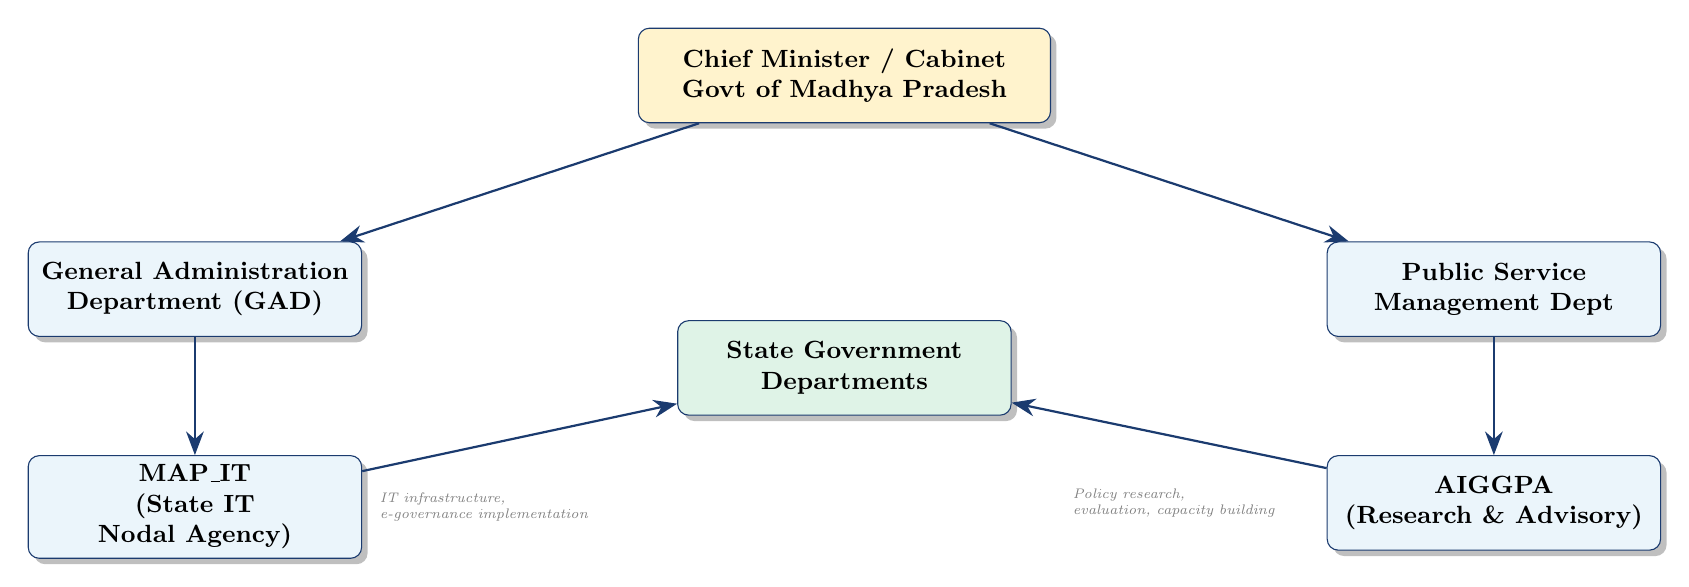
\begin{tikzpicture}[
    node distance=1.5cm and 2.5cm,
    box/.style={rectangle, rounded corners, draw=govblue, fill=boxbg, 
                text width=4cm, minimum height=1.2cm, align=center, 
                font=\small\bfseries, drop shadow},
    arrow/.style={-{Stealth[length=3mm]}, thick, govblue}
]
    % Nodes
    \node[box, fill=govgold!20, text width=5cm] (cm) {Chief Minister / Cabinet\\Govt of Madhya Pradesh};
    \node[box, below left=of cm, xshift=-1cm] (gad) {General Administration\\Department (GAD)};
    \node[box, below right=of cm, xshift=1cm] (psm) {Public Service\\Management Dept};
    \node[box, below=of gad] (mapit) {MAP\_IT\\(State IT Nodal Agency)};
    \node[box, below=of psm] (aiggpa) {AIGGPA\\(Research \& Advisory)};
    \node[box, below=2.5cm of cm, fill=accent3!15] (depts) {State Government\\Departments};
    
    % Arrows
    \draw[arrow] (cm) -- (gad);
    \draw[arrow] (cm) -- (psm);
    \draw[arrow] (gad) -- (mapit);
    \draw[arrow] (psm) -- (aiggpa);
    \draw[arrow] (mapit) -- (depts);
    \draw[arrow] (aiggpa) -- (depts);
    
    % Labels
    \node[font=\tiny\itshape, color=gray, right=0.1cm of mapit, text width=3cm] {IT infrastructure,\\e-governance implementation};
    \node[font=\tiny\itshape, color=gray, left=0.1cm of aiggpa, text width=3cm] {Policy research,\\evaluation, capacity building};
\end{tikzpicture}
\caption{Institutional architecture for governance and HR--IT integration in Madhya Pradesh. AIGGPA plays an advisory and research role, while MAP\_IT handles IT implementation.}
\label{fig:mp_architecture}
\end{figure}

\subsection{Key MP E-Governance Initiatives}

\begin{table}[H]
\centering
\caption{Madhya Pradesh  --  E-Governance Platforms (Source: MAP\_IT, MPInfo)}
\label{tab:mp_egov}
\begin{tabularx}{\textwidth}{@{}lX@{}}
\toprule
\textbf{Initiative} & \textbf{Description} \\
\midrule
MPOnline & Joint venture with TCS; centralised citizen service portal \\
e-District & G2C service delivery through Lok Sewa Kendras \\
e-Office & Paperless administrative management in state secretariat \\
Sampada 2.0 & Digital property registration (e-registration, e-stamping) \\
ITCP & Integrated Treasuries Computerisation Project \\
e-Tendering & Standardised digital procurement for all departments \\
NEVA & National e-Vidhan Application for Legislative Assembly digitisation \\
Ration Mitra & Transparent food security and ration management portal \\
SWAN & State Wide Area Network for government connectivity \\
SSDI & Spatial Data Infrastructure for GIS-based governance \\
\bottomrule
\end{tabularx}
\end{table}

\begin{notebox}[Relevance to AIGGPA]
Madhya Pradesh (\hindi{मध्य प्रदेश}) is among the \textbf{top-engagement states} for iGOT Karmayogi (Source: PIB, DD News). This demonstrates the state government's active commitment to digital capacity building, directly relevant to your internship research at AIGGPA.

\hindi{मध्य प्रदेश, आईजीओटी कर्मयोगी मंच पर सर्वाधिक सक्रिय राज्यों में शामिल है।}
\end{notebox}

% =============================================================================
\section{Theoretical \& Analytical Frameworks}

\subsection{Technology-Organization-Environment (TOE) Framework}

The most widely used model for analysing HR-IT adoption in government (Source: Emerald Insight, IAPA):

\begin{figure}[H]
\centering
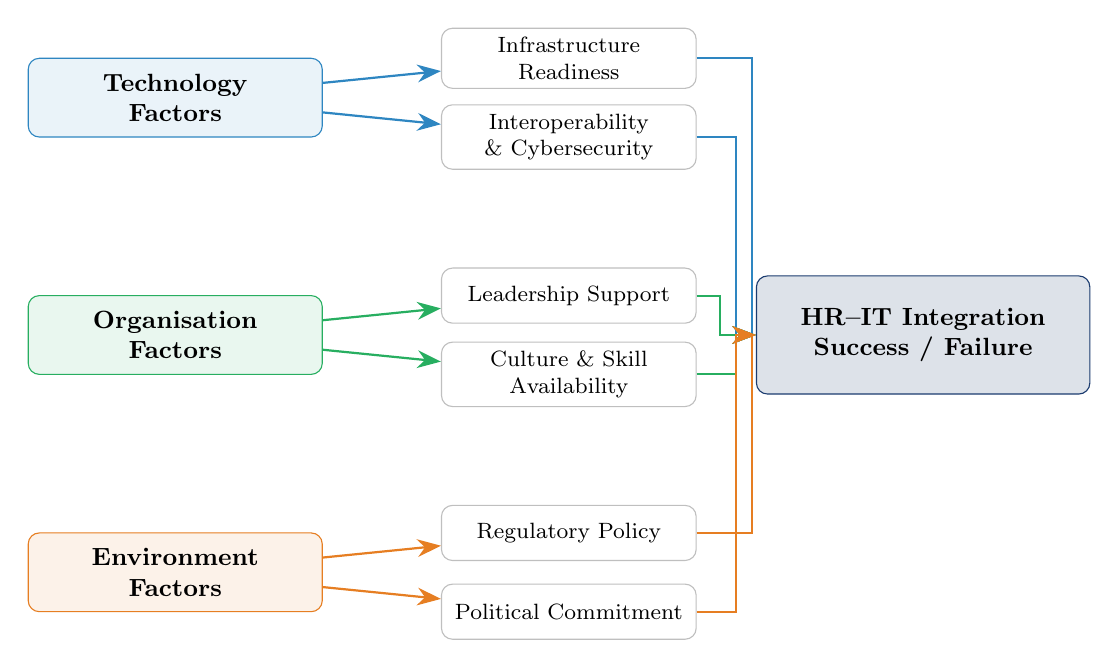
\begin{tikzpicture}[
    node distance=1.2cm and 1.5cm,
    factor/.style={rectangle, rounded corners, draw=#1, fill=#1!10, 
                   text width=3.5cm, minimum height=1cm, align=center, font=\small},
    subfactor/.style={rectangle, rounded corners, draw=gray!50, fill=white, 
                      text width=3cm, minimum height=0.7cm, align=center, font=\footnotesize},
    result/.style={rectangle, rounded corners, draw=govblue, fill=govblue!15, 
                   text width=4cm, minimum height=1.5cm, align=center, font=\small\bfseries},
    arrow/.style={-{Stealth[length=3mm]}, thick}
]
    % Main factors
    \node[factor=accent2] (tech) {\textbf{Technology}\\\textbf{Factors}};
    \node[factor=accent3, below=2cm of tech] (org) {\textbf{Organisation}\\\textbf{Factors}};
    \node[factor=accent4, below=2cm of org] (env) {\textbf{Environment}\\\textbf{Factors}};
    
    % Sub-factors
    \node[subfactor, right=1.5cm of tech, yshift=0.5cm] (t1) {Infrastructure Readiness};
    \node[subfactor, right=1.5cm of tech, yshift=-0.5cm] (t2) {Interoperability \& Cybersecurity};
    
    \node[subfactor, right=1.5cm of org, yshift=0.5cm] (o1) {Leadership Support};
    \node[subfactor, right=1.5cm of org, yshift=-0.5cm] (o2) {Culture \& Skill Availability};
    
    \node[subfactor, right=1.5cm of env, yshift=0.5cm] (e1) {Regulatory Policy};
    \node[subfactor, right=1.5cm of env, yshift=-0.5cm] (e2) {Political Commitment};
    
    % Result
    \node[result, right=5.5cm of org] (result) {HR--IT Integration\\Success / Failure};
    
    % Arrows
    \draw[arrow, accent2] (tech) -- (t1);
    \draw[arrow, accent2] (tech) -- (t2);
    \draw[arrow, accent3] (org) -- (o1);
    \draw[arrow, accent3] (org) -- (o2);
    \draw[arrow, accent4] (env) -- (e1);
    \draw[arrow, accent4] (env) -- (e2);
    
    \draw[arrow, accent2] (t1.east) -- ++(0.7,0) |- (result);
    \draw[arrow, accent2] (t2.east) -- ++(0.5,0) |- (result);
    \draw[arrow, accent3] (o1.east) -- ++(0.3,0) |- (result);
    \draw[arrow, accent3] (o2.east) -- ++(0.5,0) |- (result);
    \draw[arrow, accent4] (e1.east) -- ++(0.7,0) |- (result);
    \draw[arrow, accent4] (e2.east) -- ++(0.5,0) |- (result);
\end{tikzpicture}
\caption{Technology-Organization-Environment (TOE) Framework applied to HR--IT integration assessment. Source: Academic literature via Emerald Insight \& IAPA.}
\label{fig:toe}
\end{figure}

\subsection{2nd Administrative Reforms Commission  --  11th Report}

The landmark report titled \textbf{``Promoting e-Governance: The SMART Way Forward''} (SMART = Simple, Moral, Accountable, Responsive, Transparent) makes key recommendations relevant to HR--IT:

\begin{enumerate}
  \item \textbf{Periodic Capacity Assessment:} Every govt organisation should assess personnel's ICT capacity
  \item \textbf{Tailored Training:} Programs designed based on specific skill gap analysis
  \item \textbf{BPR First:} Business Process Re-engineering before digitisation -- don't automate bad processes
  \item \textbf{Leadership Will:} Top-level political and administrative support is essential
  \item \textbf{Incentivising Adoption:} Reward mechanisms for employees who adopt digital tools
  \item \textbf{Continuous M\&E:} Independent audits and citizen-perspective evaluations
  \item \textbf{Specialised Wings:} e-Governance units within each department
\end{enumerate}

{\footnotesize\textit{Source: Insights on India, IAS Core, MCRHRDI  --  summarising 2nd ARC, 11th Report.}}

% =============================================================================
\section{Challenges in HR--IT Integration}

\begin{figure}[H]
\centering
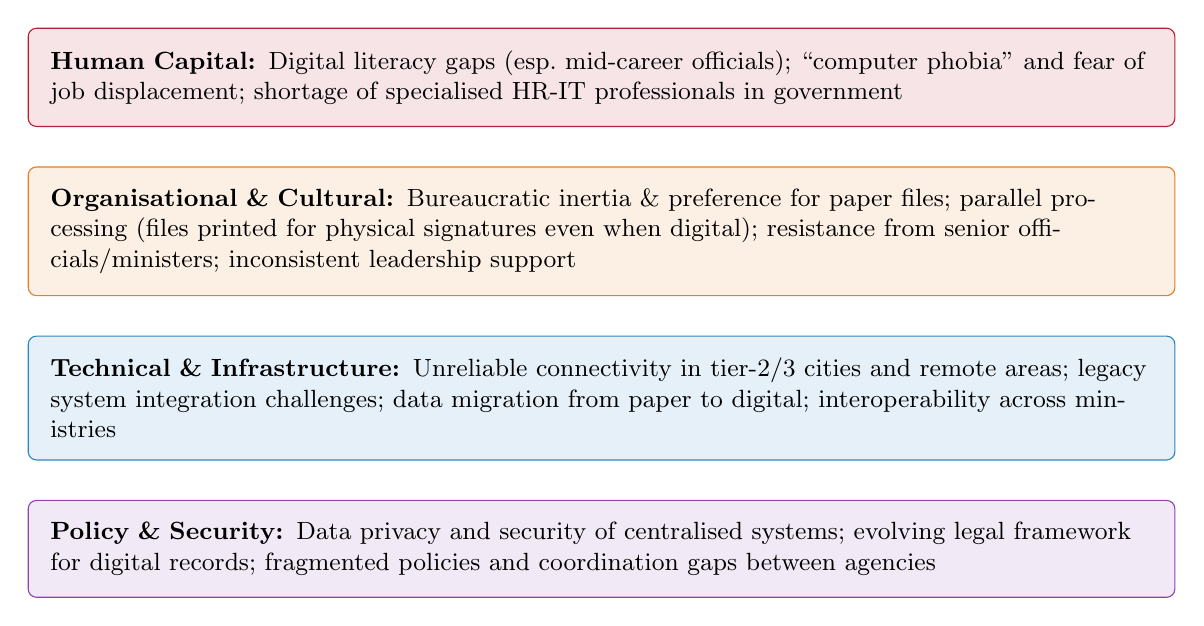
\begin{tikzpicture}[
    node distance=0.5cm,
    cat/.style={rectangle, rounded corners=3pt, draw=#1, fill=#1!12, 
                text width=14cm, minimum height=0.8cm, align=left, 
                font=\small, inner sep=8pt}
]
    \node[cat=govred] (h1) {\textbf{Human Capital:} Digital literacy gaps (esp.\ mid-career officials); ``computer phobia'' and fear of job displacement; shortage of specialised HR-IT professionals in government};
    \node[cat=accent4, below=of h1] (h2) {\textbf{Organisational \& Cultural:} Bureaucratic inertia \& preference for paper files; parallel processing (files printed for physical signatures even when digital); resistance from senior officials/ministers; inconsistent leadership support};
    \node[cat=accent2, below=of h2] (h3) {\textbf{Technical \& Infrastructure:} Unreliable connectivity in tier-2/3 cities and remote areas; legacy system integration challenges; data migration from paper to digital; interoperability across ministries};
    \node[cat=accent5, below=of h3] (h4) {\textbf{Policy \& Security:} Data privacy and security of centralised systems; evolving legal framework for digital records; fragmented policies and coordination gaps between agencies};
\end{tikzpicture}
\caption{Four categories of challenges in HR--IT integration, compiled from multiple sources including PIB, ADB, ResearchGate, and IAPA.}
\label{fig:challenges}
\end{figure}

% =============================================================================
% PART II
% =============================================================================
\newpage
\part{Assessment of Class I, II \& III Officials: Technology Usage}
\begin{center}{\Large\hindi{भाग 2: वर्ग I, II एवं III अधिकारियों का प्रौद्योगिकी उपयोग मूल्यांकन}}\end{center}

\section{Classification of Government Officials (\hindi{सरकारी अधिकारियों का वर्गीकरण})}

\begin{warningbox}[Terminology Note]
The old ``Class~I, II, III, IV'' terminology has been formally replaced by ``Group~A, B, C, D'' since 1974 via CCS~(CCA) Rules, 1965. However, the old terminology remains in widespread colloquial and official use, and is used in the internship task specification. This report uses both interchangeably. Source: Scribd (CCS Rules), Byjus, BankBazaar.
\end{warningbox}

\begin{table}[H]
\centering
\caption{Government Official Classification}
\label{tab:classification}
\begin{tabular}{@{}lllp{4.5cm}l@{}}
\toprule
\textbf{Old} & \textbf{Current} & \textbf{Nature} & \textbf{Typical Roles} & \textbf{Pay Level} \\
\midrule
Class~I & Group~A & Gazetted, Managerial & IAS, IPS, IFS, Directors, Commissioners & Level 10--18 \\
Class~II & Group~B & Gazetted/Non-Gaz., Supervisory & Section Officers, ASOs, Dy.\ Collectors & Level 6--9 \\
Class~III & Group~C & Non-Gazetted, Clerical/Technical & UDCs, LDCs, Stenographers, DEOs & Level 1--5 \\
\emph{Class~IV} & \emph{Group~D} & \emph{Support (largely merged into C)} & \emph{MTS, Peons} & \emph{Level 1} \\
\bottomrule
\end{tabular}
\end{table}

{\footnotesize\textit{Pay Levels per 7th Central Pay Commission (CPC), 2016. Source: Scribd, BajajFinserv, BankBazaar}}

% =============================================================================
\section{Technology Assessment by Class/Group (\hindi{वर्ग/समूह अनुसार प्रौद्योगिकी मूल्यांकन})}

\subsection{Class I / Group A: Senior Leadership \& Executive (\hindi{वरिष्ठ नेतृत्व})}

\textbf{Role:} Policy drivers, strategic decision-makers, platform and programme oversight.

\begin{table}[H]
\centering
\caption{Technology Usage  --  Class I / Group A Officials}
\label{tab:class1}
\begin{tabularx}{\textwidth}{@{}lcp{1cm}X@{}}
\toprule
\textbf{Tool/Platform} & \textbf{Usage} & & \textbf{Purpose} \\
\midrule
e-Office (eFile) & High & & File approval, digital signatures, policy notes \\
SPARROW / e-APAR & High & & Initiating/reviewing performance appraisals \\
e-HRMS Dashboards & High & & Workforce analytics, pendency monitoring \\
iGOT Karmayogi & Mod--High & & Strategic courses (AI, data analytics) \\
PFMS & High & & Fund monitoring, financial approvals \\
Video Conferencing (NIC) & High & & Inter-ministry coordination \\
DSC (Digital Signature) & Mandatory & & eFile approvals, document authentication \\
Email (NIC/gov.in) & Very High & & Official communication \\
\bottomrule
\end{tabularx}
\end{table}

\textbf{Key Observation:} DSCs and VPNs are now issued down to Section Officer level per CSMOP 2019. Class~I officers are mandate-givers for digital transformation. Challenge is less about tool usage and more about ensuring \textit{genuine} digital transformation vs.\ superficial compliance. Some prefer printed files for review (``parallel processing''). Source: NCGG, PIB.

\subsection{Class II / Group B: Middle Management (\hindi{मध्यम प्रबंधन})}

\textbf{Role:} The critical \textit{junction between policy and execution} -- they translate digital strategy into operational reality. Studies (Wadhwani Foundation) identify this as the \textbf{make-or-break} tier for digital initiative success.

\begin{table}[H]
\centering
\caption{Technology Usage  --  Class II / Group B Officials}
\label{tab:class2}
\begin{tabularx}{\textwidth}{@{}lcp{1cm}X@{}}
\toprule
\textbf{Tool/Platform} & \textbf{Usage} & & \textbf{Purpose} \\
\midrule
e-Office (eFile) & High & & File processing, noting, routing \\
e-HRMS & High & & Self-service + supervisory functions \\
SPARROW / e-APAR & High & & Reviewing subordinate APARs, self-assessment \\
iGOT Karmayogi & Moderate & & Functional skill development courses \\
PFMS & Mod--High & & Expenditure tracking, bill processing \\
GeM & Moderate & & Procurement processing \\
CPGRAMS & Moderate & & Departmental grievance disposal \\
Office Suite + Email & High & & Reports, presentations, communication \\
\bottomrule
\end{tabularx}
\end{table}

\textbf{Key Observation:} Many were trained in pre-digital eras and face the largest upskilling gap. iGOT engagement growing but not saturated. Critical challenge: \textit{skill gap between what they need to know and what they were originally trained for}. Source: Wadhwani Foundation, PIB.

\subsection{Class III / Group C: Operational / Clerical / Technical (\hindi{लिपिकीय/तकनीकी})}

\textbf{Role:} Day-to-day operators of digital workflows -- data entry, file movement, process execution. The largest group numerically.

\begin{table}[H]
\centering
\caption{Technology Usage  --  Class III / Group C Officials}
\label{tab:class3}
\begin{tabularx}{\textwidth}{@{}lcp{1cm}X@{}}
\toprule
\textbf{Tool/Platform} & \textbf{Usage} & & \textbf{Purpose} \\
\midrule
e-Office (eFile) & Moderate & & Creating receipts, initiating files \\
e-HRMS (ESS) & Moderate & & Leave applications, personal data views \\
Basic Office Suite & Mod--High & & Word processing, data entry, spreadsheets \\
AEBAS (Biometric) & High* & & Aadhaar-based attendance (*where deployed) \\
Dept-specific portals & Variable & & Data entry, record management \\
iGOT Karmayogi & Low--Mod & & Basic/compliance training courses \\
Email & Moderate & & Limited; many still rely on physical \textit{dak} \\
\bottomrule
\end{tabularx}
\end{table}

\textbf{Key Observation:} Most significant digital divide exists here. Adoption is heavily dependent on: hardware availability (many share computers), internet connectivity (especially in district/taluk offices), department mandates, and individual comfort level. Many still maintain parallel paper records. Source: ADB, DARPG, academic literature.

% =============================================================================
\section{Comparative Assessment Matrix}

\begin{table}[H]
\centering
\caption{Cross-Class Technology Adoption Comparison}
\label{tab:comparison}
\begin{tabularx}{\textwidth}{@{}Xlll@{}}
\toprule
\textbf{Parameter} & \textbf{Class I (Grp A)} & \textbf{Class II (Grp B)} & \textbf{Class III (Grp C)} \\
\midrule
Primary Tech Role & Strategic / Policy & Supervisory / Translation & Operational / Execution \\
Digital Literacy & High & Moderate & Low--Moderate \\
Hardware Access & Dedicated laptop/desktop & Dedicated desktop & Often shared / outdated \\
Connectivity & Reliable (central) & Mostly reliable & Variable (field offices) \\
e-Office Usage & Daily (approvals) & Daily (processing) & Periodic (data entry) \\
iGOT Engagement & AI/strategic courses & Functional courses & Basic/compliance \\
DSC Usage & Mandatory & Common & Rare \\
Change Resistance & Low (hybrid pref.) & Moderate & High \\
\textbf{Key Barrier} & Vision, parallel systems & Skill gaps & Infrastructure, literacy \\
\bottomrule
\end{tabularx}
\end{table}

%  --  Class-wise Radar/Comparison Bar Chart  -- 
\begin{figure}[H]
\centering
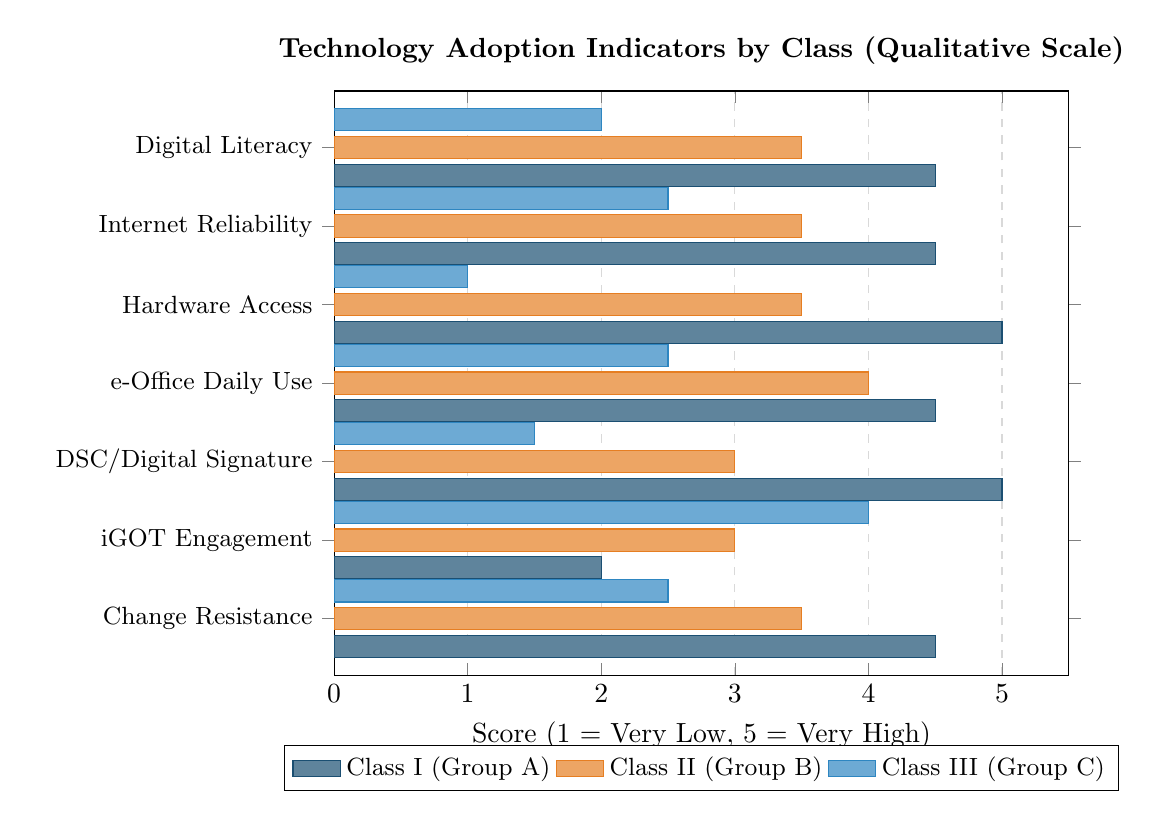
\begin{tikzpicture}
\begin{axis}[
    title={\textbf{Technology Adoption Indicators by Class (Qualitative Scale)}},
    width=0.9\textwidth,
    height=9cm,
    xbar,
    bar width=8pt,
    xlabel={Score (1 = Very Low, 5 = Very High)},
    xmin=0, xmax=5.5,
    ytick={1,2,3,4,5,6,7},
    yticklabels={
        {Change Resistance},
        {iGOT Engagement},
        {DSC/Digital Signature},
        {e-Office Daily Use},
        {Hardware Access},
        {Internet Reliability},
        {Digital Literacy}
    },
    y tick label style={font=\small, text width=3.5cm, align=right},
    legend style={at={(0.5,-0.12)}, anchor=north, legend columns=3, font=\small},
    ymajorgrids=false,
    xmajorgrids=true,
    grid style={dashed, gray!30},
    enlarge y limits=0.12,
    area legend,
]
% Class I
\addplot[fill=accent1!70, draw=accent1] coordinates {(4.5,7) (4.5,6) (5,5) (4.5,4) (5,3) (2,2) (4.5,1)};
% Class II
\addplot[fill=accent4!70, draw=accent4] coordinates {(3.5,7) (3.5,6) (3.5,5) (4,4) (3,3) (3,2) (3.5,1)};
% Class III
\addplot[fill=accent2!70, draw=accent2] coordinates {(2,7) (2.5,6) (1,5) (2.5,4) (1.5,3) (4,2) (2.5,1)};
\legend{Class I (Group A), Class II (Group B), Class III (Group C)}
\end{axis}
\end{tikzpicture}
\caption{Qualitative comparison of technology adoption indicators across the three classes. Scores are on a 1--5 scale derived from secondary literature analysis. Note: ``Change Resistance'' is reverse-scored -- higher score = lower resistance. Sources: PIB, Wadhwani Foundation, ADB, DARPG, NIC, NCGG.}
\label{fig:class_comparison}
\end{figure}

% =============================================================================
\section{Key Findings from National Assessments}

\subsection{NeSDA (National e-Service Delivery Assessment / \hindi{राष्ट्रीय ई-सेवा वितरण मूल्यांकन})}

\begin{sourcebox}[NeSDA Facts]
\begin{itemize}[leftmargin=1cm]
  \item Published by DARPG; tracks e-service delivery maturity across States/UTs
  \item By November 2024: \textbf{$\sim$78\% saturation} of mandatory e-services across states
  \item Focus sectors: Local Governance, Finance, Education, Environment, Labour, Social Welfare, Tourism
  \item Monthly ``NeSDA Way Forward'' reports published on DARPG website
  \item States pushed toward unified/centralised service delivery portals and faceless services
\end{itemize}
\textit{Source: DARPG official website, PIB, S3WaaS.gov.in}
\end{sourcebox}

\subsection{iGOT Data as a Proxy for Technology Engagement}

\begin{figure}[H]
\centering
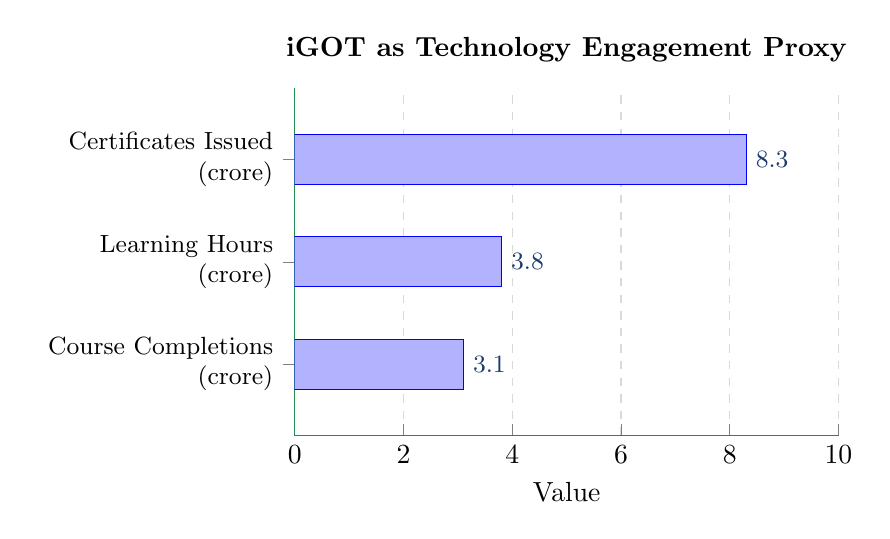
\begin{tikzpicture}
\begin{axis}[
    title={\textbf{iGOT as Technology Engagement Proxy}},
    width=0.7\textwidth,
    height=6cm,
    xbar,
    bar width=18pt,
    xlabel={Value},
    ytick={1,2,3},
    yticklabels={
        {Course Completions\\(crore)},
        {Learning Hours\\(crore)},
        {Certificates Issued\\(crore)}
    },
    y tick label style={font=\small, text width=3cm, align=right},
    xmin=0, xmax=10,
    nodes near coords,
    every node near coord/.append style={font=\small\bfseries, color=govblue},
    fill=accent3!65,
    draw=accent3!80!black,
    axis lines*=left,
    xmajorgrids=true,
    grid style={dashed, gray!30},
    enlarge y limits=0.35,
]
\addplot coordinates {(8.3,3) (3.8,2) (3.1,1)};
\end{axis}
\end{tikzpicture}
\caption{iGOT Karmayogi engagement metrics (cumulative as of March 2026). Source: PIB, 27 March 2026.}
\label{fig:igot_engagement}
\end{figure}

% =============================================================================
\section{HR--IT Integration Ecosystem  --  Architectural Overview}

\begin{figure}[H]
\centering
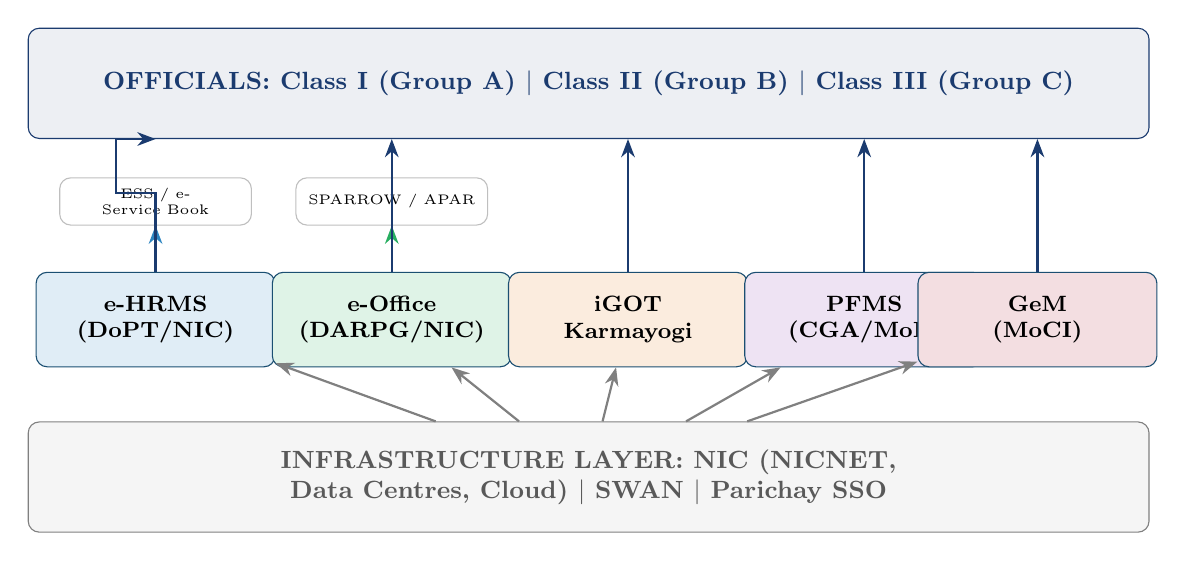
\begin{tikzpicture}[
    node distance=1cm and 1.5cm,
    platform/.style={rectangle, rounded corners, draw=accent1, fill=accent1!8, 
                     text width=2.8cm, minimum height=1.2cm, align=center, 
                     font=\footnotesize\bfseries},
    layer/.style={rectangle, rounded corners, draw=#1, fill=#1!8, 
                  text width=14cm, minimum height=1.4cm, align=center, 
                  font=\small\bfseries},
]
    % Infrastructure Layer
    \node[layer=gray] (infra) at (0,0) {\textcolor{gray!70!black}{INFRASTRUCTURE LAYER: NIC (NICNET, Data Centres, Cloud) $\vert$ SWAN $\vert$ Parichay SSO}};
    
    % Platforms Layer
    \node[platform, fill=accent2!15] (ehrms) at (-5.5,2) {e-HRMS\\(DoPT/NIC)};
    \node[platform, fill=accent3!15] (eoffice) at (-2.5,2) {e-Office\\(DARPG/NIC)};
    \node[platform, fill=accent4!15] (igot) at (0.5,2) {iGOT\\Karmayogi};
    \node[platform, fill=accent5!15] (pfms) at (3.5,2) {PFMS\\(CGA/MoF)};
    \node[platform, fill=govred!15] (gem) at (5.7,2) {GeM\\(MoCI)};
    
    % Sub-modules
    \node[rectangle, rounded corners, draw=gray!50, fill=white, text width=2.2cm, minimum height=0.6cm, align=center, font=\tiny] (sparrow) at (-2.5,3.5) {SPARROW / APAR};
    \node[rectangle, rounded corners, draw=gray!50, fill=white, text width=2.2cm, minimum height=0.6cm, align=center, font=\tiny] (ess) at (-5.5,3.5) {ESS / e-Service Book};
    
    % User Layer
    \node[layer=govblue] (users) at (0,5) {\textcolor{govblue}{OFFICIALS: Class I (Group A) $\vert$ Class II (Group B) $\vert$ Class III (Group C)}};
    
    % Arrows
    \draw[-{Stealth}, thick, gray] (infra) -- (ehrms);
    \draw[-{Stealth}, thick, gray] (infra) -- (eoffice);
    \draw[-{Stealth}, thick, gray] (infra) -- (igot);
    \draw[-{Stealth}, thick, gray] (infra) -- (pfms);
    \draw[-{Stealth}, thick, gray] (infra) -- (gem);
    
    \draw[-{Stealth}, thick, accent2] (ehrms) -- (ess);
    \draw[-{Stealth}, thick, accent3] (eoffice) -- (sparrow);
    
    \draw[-{Stealth}, thick, govblue] (ehrms.north) -- ++(0,1) -- ++(-0.5,0) |- (users.south -| ehrms);
    \draw[-{Stealth}, thick, govblue] (eoffice) -- (users.south -| eoffice);
    \draw[-{Stealth}, thick, govblue] (igot) -- (users.south -| igot);
    \draw[-{Stealth}, thick, govblue] (pfms) -- (users.south -| pfms);
    \draw[-{Stealth}, thick, govblue] (gem) -- (users.south -| gem);
\end{tikzpicture}
\caption{Architectural overview of the government HR--IT ecosystem, showing infrastructure, platform, and user layers.}
\label{fig:ecosystem}
\end{figure}

% =============================================================================
\section{Recommendations for Internship Research}

\subsection{For HR--IT Integration Research at AIGGPA (\hindi{एआईजीजीपीए में अनुसंधान})}

\begin{enumerate}
  \item \textbf{Gap Analysis:} Map which MP departments have adopted e-Office, e-HRMS, and iGOT -- and which have not
  \item \textbf{Integration Maturity Model:} Create a framework rating departments on a 1--5 scale of HR--IT integration maturity
  \item \textbf{Case Studies:} Document 2--3 departments where HR--IT integration is working well, and 2--3 where it lags -- identify root causes
  \item \textbf{Policy Brief:} Draft a policy advisory for the MP government on accelerating HR--IT convergence
\end{enumerate}

\subsection{For Technology Assessment of Officials (\hindi{अधिकारियों का प्रौद्योगिकी मूल्यांकन})}

\begin{enumerate}
  \item \textbf{Survey Design:} Create a structured questionnaire targeting Class I/II/III officials on technology usage, comfort, barriers, and training needs
  \item \textbf{Department Sampling:} Select 5--6 departments across sectors for heterogeneity
  \item \textbf{Field Observations:} Visit district offices to observe \textit{actual} technology usage vs.\ claimed usage
  \item \textbf{NeSDA Benchmarking:} Compare MP's performance against national NeSDA benchmarks
  \item \textbf{Training Needs Assessment:} Map skill gaps to iGOT courses and recommend targeted interventions
\end{enumerate}

% =============================================================================
% PART III
% =============================================================================
\newpage
\part{Primary Research Conceptualization Framework}
\begin{center}{\Large\hindi{भाग 3: प्राथमिक अनुसंधान की रूपरेखा -- गवटेक अपनाने का सूचकांक}}\end{center}

\begin{notebox}[Purpose of This Section]
This section outlines the {\bfseries conceptual architecture} for the primary research phase of this internship. It defines what will be measured, how respondents will be categorised, which departments will be studied, and the methodology that will translate raw data into actionable insight. This is not a literature review -- it is a {\bfseries research design blueprint} ({\hindi{अनुसंधान डिज़ाइन का खाका}}).
\end{notebox}

% =============================================================================
\section{The Three-Tier Adoption Model (\hindi{तीन-स्तरीय अपनाने का मॉडल})}

The core diagnostic framework classifies every government employee into one of three tiers based on their relationship with official IT tools:

\begin{figure}[H]
\centering
\begin{tikzpicture}[
    node distance=0.8cm and 2cm,
    tier/.style={rectangle, rounded corners=6pt, draw=#1, fill=#1!12,
                 text width=4.2cm, minimum height=3.5cm, align=center,
                 font=\small, inner sep=10pt, drop shadow},
    arrow/.style={-{Stealth[length=3mm]}, thick, gray!60}
]
    % Three tiers
    \node[tier=accent3] (t1) {
        {\Large\bfseries\textcolor{accent3}{TIER 1}}\\[4pt]
        {\bfseries Active Adopters}\\[2pt]
        \hindi{सक्रिय उपयोगकर्ता}\\[6pt]
        \footnotesize Uses IT tools daily;\\
        \footnotesize e-Office, e-HRMS,\\
        \footnotesize iGOT integrated\\
        \footnotesize into workflow\\[6pt]
        \footnotesize\textit{Intervention:}\\
        \footnotesize\textbf{Optimise \& Retain}
    };

    \node[tier=accent4, right=2.5cm of t1] (t2) {
        {\Large\bfseries\textcolor{accent4}{TIER 2}}\\[4pt]
        {\bfseries Hesitant Users}\\[2pt]
        \hindi{संकोची उपयोगकर्ता}\\[6pt]
        \footnotesize Aware of tools,\\
        \footnotesize possibly trained,\\
        \footnotesize but defaults to\\
        \footnotesize paper/manual\\[6pt]
        \footnotesize\textit{Intervention:}\\
        \footnotesize\textbf{Motivate + Remove}\\
        \footnotesize\textbf{Barriers}
    };

    \node[tier=govred, right=2.5cm of t2] (t3) {
        {\Large\bfseries\textcolor{govred}{TIER 3}}\\[4pt]
        {\bfseries Unaware Non-Users}\\[2pt]
        \hindi{अनजान गैर-उपयोगकर्ता}\\[6pt]
        \footnotesize No exposure,\\
        \footnotesize no training,\\
        \footnotesize no access;\\
        \footnotesize ``Does not even know''\\[6pt]
        \footnotesize\textit{Intervention:}\\
        \footnotesize\textbf{Awareness +}\\
        \footnotesize\textbf{Training + Hardware}
    };

    % Arrows indicating diagnostics
    \draw[arrow] (t1.south) -- ++(0,-0.8) node[below, font=\footnotesize\itshape, text width=3cm, align=center] {Measure usage depth};
    \draw[arrow] (t2.south) -- ++(0,-0.8) node[below, font=\footnotesize\itshape, text width=3cm, align=center] {Identify barriers \& motivators};
    \draw[arrow] (t3.south) -- ++(0,-0.8) node[below, font=\footnotesize\itshape, text width=3cm, align=center] {Map awareness gaps};

    % Overarching label
    \node[above=0.8cm of t2, font=\bfseries\large\color{govblue}] {GovTech Adoption Index -- Tier Classification};
\end{tikzpicture}
\caption{The Three-Tier Adoption Model. Each government employee is classified based on their IT tool awareness, ability, and actual usage. The model is derived from field observations referenced in handwritten research notes and aligned with iGOT's ASK (Attitude, Skills, Knowledge) framework.}
\label{fig:three_tier}
\end{figure}

\textbf{The central research question:} \textit{Within each department, what is the distribution of employees across these three tiers -- and what demographic, organisational, and infrastructure factors drive that distribution?}

% =============================================================================
\section{Department Selection (\hindi{विभाग चयन})}

\subsection{Selection Criteria}

Departments are selected along two axes -- \textbf{digitisation maturity} and \textbf{public interaction intensity} -- to maximise comparative insight:

\begin{figure}[H]
\centering
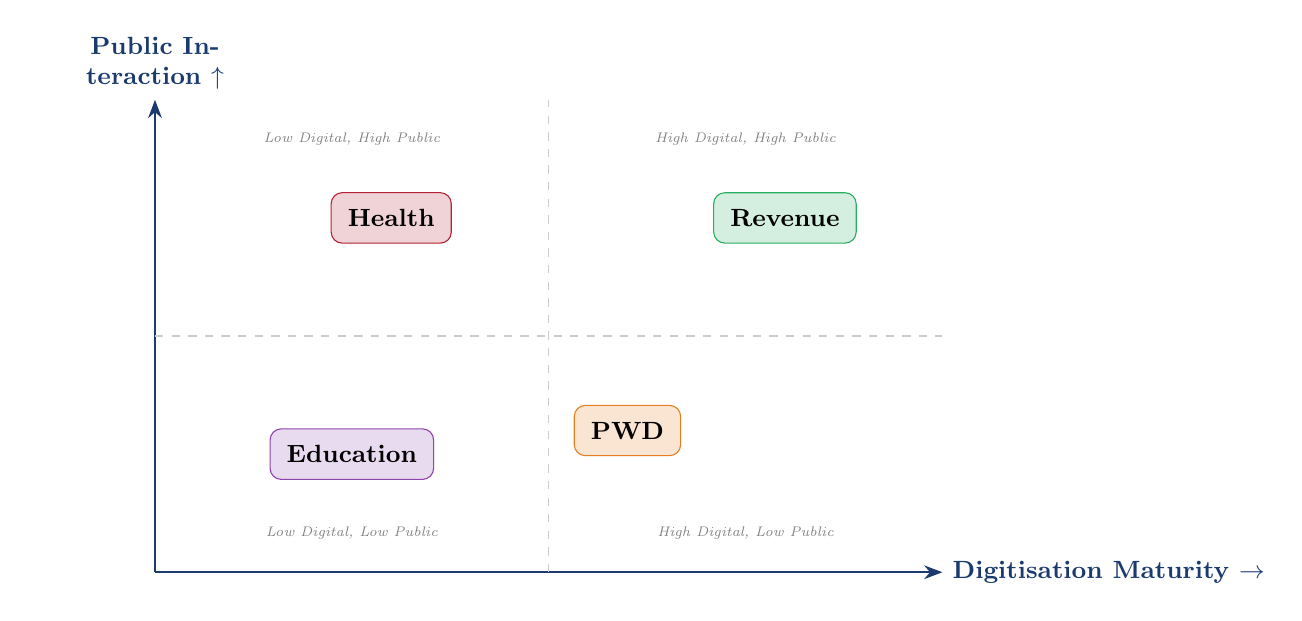
\begin{tikzpicture}
    % Axes
    \draw[-{Stealth}, thick, govblue] (0,0) -- (10,0) node[right, font=\small\bfseries] {Digitisation Maturity $\rightarrow$};
    \draw[-{Stealth}, thick, govblue] (0,0) -- (0,6) node[above, font=\small\bfseries, text width=3cm, align=center] {Public Interaction $\uparrow$};

    % Quadrant labels
    \node[font=\tiny\itshape, color=gray] at (2.5,5.5) {Low Digital, High Public};
    \node[font=\tiny\itshape, color=gray] at (7.5,5.5) {High Digital, High Public};
    \node[font=\tiny\itshape, color=gray] at (2.5,0.5) {Low Digital, Low Public};
    \node[font=\tiny\itshape, color=gray] at (7.5,0.5) {High Digital, Low Public};

    % Dashed quadrant lines
    \draw[dashed, gray!40] (5,0) -- (5,6);
    \draw[dashed, gray!40] (0,3) -- (10,3);

    % Departments
    \node[rectangle, rounded corners, fill=govred!20, draw=govred, font=\small\bfseries, inner sep=6pt] at (3,4.5) {Health};
    \node[rectangle, rounded corners, fill=accent3!20, draw=accent3, font=\small\bfseries, inner sep=6pt] at (8,4.5) {Revenue};
    \node[rectangle, rounded corners, fill=accent5!20, draw=accent5, font=\small\bfseries, inner sep=6pt] at (2.5,1.5) {Education};
    \node[rectangle, rounded corners, fill=accent4!20, draw=accent4, font=\small\bfseries, inner sep=6pt] at (6,1.8) {PWD};
\end{tikzpicture}
\caption{Department selection matrix: 2$\times$2 placement based on digitisation maturity and public interaction intensity. This ensures maximum comparative diversity.}
\label{fig:dept_matrix}
\end{figure}

\subsection{The 4 Selected Departments}

\begin{table}[H]
\centering
\caption{Selected Departments for Primary Research}
\label{tab:dept_selection}
\begin{tabularx}{\textwidth}{@{}clXl@{}}
\toprule
\textbf{\#} & \textbf{Department} & \textbf{Selection Rationale} & \textbf{Key IT Tools} \\
\midrule
1 & \makecell[l]{Revenue / Land Records\\(\hindi{भू-अभिलेख})} & Highest digital transaction volume in any state government department; direct citizen interface via land records & Bhulekh, RCMS, e-District, e-Office \\
\addlinespace
2 & \makecell[l]{Public Works / PWD\\(\hindi{लोक निर्माण विभाग})} & Engineering workforce transitioning from manual tenders to e-tendering; moderate digitisation with low public interaction & e-Tendering, e-Office, PFMS \\
\addlinespace
3 & \makecell[l]{Health / Public Hospitals\\(\hindi{स्वास्थ्य विभाग})} & Large frontline workforce with high public interaction; inventory and patient record management challenges & HMIS, Ayushman Bharat, CoWIN backend \\
\addlinespace
4 & \makecell[l]{School Education\\(\hindi{स्कूल शिक्षा विभाग})} & Highest volume of Group C employees; direct LMS engagement via iGOT/Diksha; lowest expected IT maturity & Diksha, iGOT, UDISE+ \\
\bottomrule
\end{tabularx}
\end{table}

\begin{warningbox}[Flexibility Note]
If access to any of the above departments is not feasible during the internship, alternative departments with similar characteristics include: Finance/Treasury (high IT, replaces Revenue), Agriculture (low IT, replaces Education), Urban Development (medium IT, replaces PWD), and Women \& Child Development (variable IT, replaces Health).
\end{warningbox}

% =============================================================================
\section{Demographics \& Categorisation Strategy (\hindi{जनसांख्यिकी एवं वर्गीकरण})}

Respondents will be classified across six demographic dimensions to enable multi-variate analysis of IT adoption patterns.

\subsection{Gender (\hindi{लिंग})}

\begin{table}[H]
\centering
\caption{Gender Categorisation}
\label{tab:demo_gender}
\begin{tabularx}{\textwidth}{@{}llX@{}}
\toprule
\textbf{Category} & \textbf{Metric} & \textbf{Analytical Purpose} \\
\midrule
Male & \multirow{3}{*}{\shortstack[l]{Gender Parity Index\\= (Female adoption rate /\\Male adoption rate)}} & Baseline comparison \\
Female & & Check if digital literacy programmes reach equitably; identify gender-specific barriers (e.g., mobile access, training timing) \\
Prefer not to say & & Research ethics compliance \\
\bottomrule
\end{tabularx}
\end{table}

\textbf{Key metric:} \textit{Gender Parity Index (GPI) in IT adoption}. A score of 1.0 indicates perfect parity; $<$1.0 indicates female under-adoption; $>$1.0 indicates male under-adoption.

\subsection{Age Groups (\hindi{आयु वर्ग})}

\begin{table}[H]
\centering
\caption{Age Group Categorisation with Adoption Hypothesis}
\label{tab:demo_age}
\begin{tabularx}{\textwidth}{@{}llX@{}}
\toprule
\textbf{Age Bracket} & \textbf{Label} & \textbf{Hypothesis} \\
\midrule
$<$ 30 years & Digital Native Entrant & High comfort with technology; likely frustrated by legacy systems and slow institutional adoption \\
30--40 years & Early-Mid Career & Moderate comfort; willing to learn if properly incentivised through training and career benefits \\
41--50 years & Mid-Career Transition & The primary ``knows but not using'' cohort -- largest intervention target with highest ROI potential \\
51+ years & Late-Career / Pre-Retirement & Likely the ``does not even know'' group; highest change resistance; shortest payback window \\
\bottomrule
\end{tabularx}
\end{table}

\textbf{Key metric:} \textit{Age-Adoption Correlation Coefficient} -- does IT usage drop linearly with age, or is there a discontinuous ``cliff'' at a specific age threshold?

\subsection{Role / Grade Level (\hindi{पद/समूह स्तर})}

Grade-level categorisation follows the Class I/II/III framework already established in Part~II (Tables~\ref{tab:class1}--\ref{tab:class3}). The primary research will \textbf{validate} those secondary findings.

\begin{table}[H]
\centering
\caption{Grade-Level Research Focus}
\label{tab:demo_grade}
\begin{tabularx}{\textwidth}{@{}llX@{}}
\toprule
\textbf{Classification} & \textbf{Expected Tier} & \textbf{Research Focus} \\
\midrule
Class I / Group A & Tier 1 (Active) & Validate if ``parallel processing'' (printing digital files) occurs; assess strategic vision for IT \\
Class II / Group B & Tier 1--2 (Mixed) & Identify the ``make-or-break'' junction -- do they translate digital policy into execution? \\
Class III / Group C & Tier 2--3 (Hesitant/Unaware) & Measure infrastructure barriers; quantify hardware sharing; assess training accessibility \\
\bottomrule
\end{tabularx}
\end{table}

\subsection{Education Level (\hindi{शैक्षिक स्तर})}

\begin{table}[H]
\centering
\caption{Education Level Categories}
\label{tab:demo_education}
\begin{tabularx}{\textwidth}{@{}lX@{}}
\toprule
\textbf{Level} & \textbf{Analytical Purpose} \\
\midrule
Up to 12th / Diploma & May correlate with lower digital confidence; baseline category \\
Graduate (BA/BSc/BCom) & Standard level; baseline digital exposure through university \\
Post-Graduate (MA/MBA/MTech) & Higher expected IT comfort; validate assumption \\
Professional / Technical (CA, Engineering) & Expected high tool fluency; test if domain expertise translates to govt IT adoption \\
\bottomrule
\end{tabularx}
\end{table}

\subsection{Location / Posting Type (\hindi{पोस्टिंग स्थान})}

\begin{table}[H]
\centering
\caption{Posting Location Categories}
\label{tab:demo_location}
\begin{tabularx}{\textwidth}{@{}lX@{}}
\toprule
\textbf{Location Type} & \textbf{Infrastructure Characteristics} \\
\midrule
State Capital (Bhopal) & Best infrastructure, highest mandate compliance, dedicated hardware \\
District Headquarters & Moderate infrastructure, variable compliance, some shared hardware \\
Tehsil / Block Level & Poor connectivity, shared/outdated hardware, highest expected ``digital gap'' \\
Field / Mobile Posting & Health workers, revenue inspectors; rely on personal mobile devices \\
\bottomrule
\end{tabularx}
\end{table}

\subsection{Years of Service (\hindi{सेवा अवधि})}

\begin{table}[H]
\centering
\caption{Service Duration Categories}
\label{tab:demo_service}
\begin{tabularx}{\textwidth}{@{}lX@{}}
\toprule
\textbf{Bracket} & \textbf{Relevance} \\
\midrule
0--5 years & Recent recruit -- trained in the digital era? Does institutional onboarding include IT tools? \\
6--15 years & Mid-service -- experienced the analogue-to-digital transition firsthand \\
16--25 years & Senior -- likely trained pre-digital; measures effectiveness of mid-career upskilling \\
26+ years & Near-retirement -- highest inertia risk; lowest institutional ROI for training investment \\
\bottomrule
\end{tabularx}
\end{table}

% =============================================================================
\section{Metrics \& Measurement Framework (\hindi{मापदंड एवं मापन रूपरेखा})}

\subsection{Quantitative Metrics (Hard Data)}

\begin{table}[H]
\centering
\caption{Quantitative Metrics for IT Adoption Measurement}
\label{tab:metrics_quant}
\begin{tabularx}{\textwidth}{@{}clXl@{}}
\toprule
\textbf{\#} & \textbf{Metric} & \textbf{Formula / Data Source} & \textbf{Unit} \\
\midrule
1 & Digital Penetration Rate & (Tasks completed digitally / Total tasks) $\times$ 100 & \% \\
2 & Platform Login Frequency & Average logins per user per month (from e-Office / e-HRMS logs) & logins/month \\
3 & Task Completion Time & Average time for digital process vs.\ manual benchmark & hours \\
4 & iGOT Course Completion Rate & (Courses completed / Courses assigned) $\times$ 100 & \% \\
5 & Training ROI & Post-training IT usage score $-$ Pre-training IT usage score & $\Delta$ score \\
6 & Hardware Availability Ratio & (Functional computers / Employees in the office) $\times$ 100 & \% \\
7 & Connectivity Uptime & \% of working hours with functional internet & \% \\
\bottomrule
\end{tabularx}
\end{table}

\subsection{Qualitative Metrics (Survey-Derived)}

\begin{table}[H]
\centering
\caption{Qualitative Metrics -- Likert Scale and Rank-Order Items}
\label{tab:metrics_qual}
\begin{tabularx}{\textwidth}{@{}clXl@{}}
\toprule
\textbf{\#} & \textbf{Metric} & \textbf{Survey Item (Illustrative)} & \textbf{Scale} \\
\midrule
8 & Digital Confidence Score & ``I feel confident using e-Office for my daily work'' & Likert 1--5 \\
9 & Frustration Score & ``I find government IT tools difficult to use'' & Likert 1--5 (rev.) \\
10 & Awareness Index & ``I know about the following platforms: [checklist]'' & Count 0--10 \\
11 & Willingness to Adopt & ``I would use IT tools more if trained properly'' & Likert 1--5 \\
12 & Supervisor Mandate & ``My supervisor encourages digital tool usage'' & Likert 1--5 \\
13 & Barrier Ranking & ``Rank: No hardware / No training / No internet / No need / Fear'' & Rank order \\
14 & Paper Dependency Score & ``How often do you print digital files for physical signatures?'' & Frequency \\
15 & Peer Influence & ``My colleagues' IT usage influences my own'' & Likert 1--5 \\
\bottomrule
\end{tabularx}
\end{table}

\subsection{The Composite GovTech Adoption Index}

The individual metrics are combined into a single department-level {\bfseries composite score} enabling direct cross-department comparison:

\begin{sourcebox}[Composite Index Formula]
\begin{equation*}
\text{GovTech Adoption Index} = w_1(\text{DP}) + w_2(\text{LF}) + w_3(\text{CS}) + w_4(\text{AI}) + w_5(\text{HR}) - w_6(\text{FS})
\end{equation*}

\noindent Where:
\begin{itemize}[leftmargin=1cm, itemsep=2pt]
  \item DP = Digital Penetration Rate (normalised 0--1)
  \item LF = Platform Login Frequency (normalised 0--1)
  \item CS = Digital Confidence Score (mean Likert, normalised 0--1)
  \item AI = Awareness Index (normalised 0--1)
  \item HR = Hardware Availability Ratio (normalised 0--1)
  \item FS = Frustration Score (normalised 0--1; \textbf{subtracted} as it is an inverse indicator)
  \item $w_1 \ldots w_6$ = Weights determined via factor analysis or Delphi-method expert consultation
\end{itemize}

\noindent\textbf{Output:} Each department receives a score on a \textbf{0--100 scale}, enabling direct comparison and ranking.
\end{sourcebox}

%  --  Expected Index Distribution Chart  --
\begin{figure}[H]
\centering
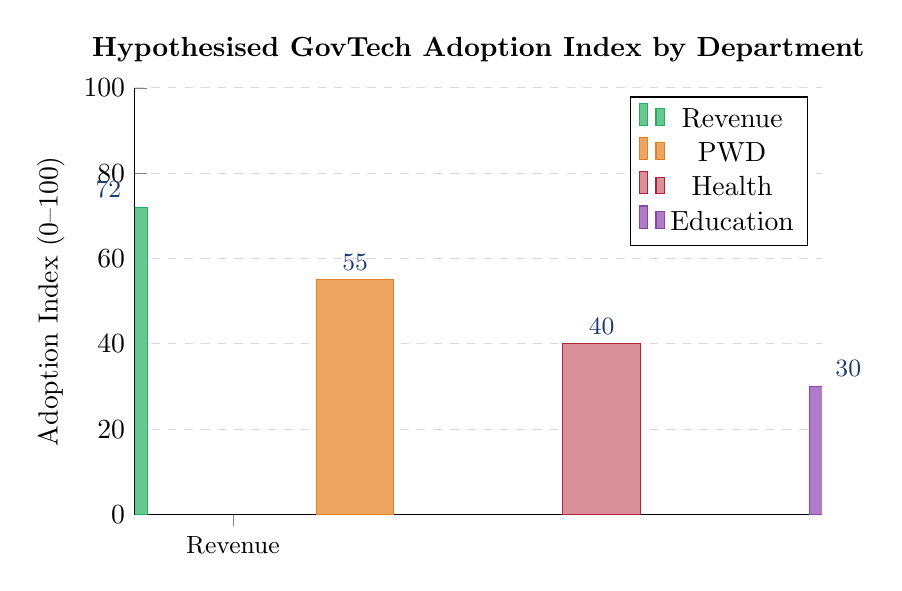
\begin{tikzpicture}
\begin{axis}[
    title={\textbf{Hypothesised GovTech Adoption Index by Department}},
    width=0.85\textwidth,
    height=7cm,
    ybar,
    bar width=28pt,
    ylabel={Adoption Index (0--100)},
    symbolic x coords={Revenue, PWD, Health, Education},
    xtick=data,
    ymin=0, ymax=100,
    nodes near coords,
    every node near coord/.append style={font=\small\bfseries, color=govblue},
    axis lines*=left,
    ymajorgrids=true,
    grid style={dashed, gray!30},
    x tick label style={font=\small},
    enlarge x limits=0.2,
]
\addplot[fill=accent3!70, draw=accent3] coordinates {(Revenue, 72)};
\addplot[fill=accent4!70, draw=accent4] coordinates {(PWD, 55)};
\addplot[fill=govred!50, draw=govred] coordinates {(Health, 40)};
\addplot[fill=accent5!70, draw=accent5] coordinates {(Education, 30)};
\legend{Revenue, PWD, Health, Education}
\end{axis}
\end{tikzpicture}
\caption{Hypothesised GovTech Adoption Index scores for the four selected departments. These are {\itshape pre-research estimates} based on the secondary research in Part~I and Part~II. Primary research will validate or revise these figures. Revenue is expected to score highest due to its advanced digitisation (Bhulekh, RCMS); Education is expected to score lowest due to infrastructure constraints and large Group~C workforce.}
\label{fig:hypothesised_index}
\end{figure}

% =============================================================================
\section{Research Implementation Strategy (\hindi{अनुसंधान कार्यान्वयन रणनीति})}

\subsection{Sampling Design}

\begin{table}[H]
\centering
\caption{Sampling Plan}
\label{tab:sampling}
\begin{tabularx}{\textwidth}{@{}lX@{}}
\toprule
\textbf{Parameter} & \textbf{Value} \\
\midrule
Total target respondents & $\sim$120 (30 per department $\times$ 4 departments) \\
Sampling method & Purposive + Stratified Random \\
Stratification variables & Grade (Group A/B/C), Gender, Age bracket \\
Minimum per cell & 5 respondents (e.g., 5 female Group C employees per department) \\
Survey language & Bilingual -- Hindi (\hindi{हिन्दी}) primary, English secondary \\
Survey mode & Paper + Digital (Google Forms / KoboToolbox for offline compatibility) \\
\bottomrule
\end{tabularx}
\end{table}

\subsection{Five-Step Data Collection Protocol}

\begin{enumerate}[label=\textbf{Step \Alph*:}, leftmargin=2.5cm]

  \item \textbf{Desk Audit (Week 1--2)} \\
  Collect login/usage data from department IT cells (e-Office, e-HRMS dashboards). Obtain official employee rosters with age, grade, and posting data. Map which IT tools each department officially mandates.

  \item \textbf{Structured Survey (Week 3--5)} \\
  Deploy the bilingual questionnaire covering all 15 metrics (Tables~\ref{tab:metrics_quant}~\&~\ref{tab:metrics_qual}). Administer via paper at field offices and digitally at headquarters. Target: 120+ completed responses.

  \item \textbf{Observation / Shadowing (Week 4--6)} \\
  Shadow 2 employees per department for half a day each (8 sessions total). Observe: do they use e-Office or print files? Do they check iGOT? What is their default workflow? Capture the ``parallel processing'' behaviour identified in the secondary research.

  \item \textbf{Key Informant Interviews (Week 5--7)} \\
  Conduct 1--2 semi-structured interviews with senior officials (Group A) per department (4--8 total). Focus: department-level IT mandates, resistance patterns, budget constraints, training efficacy. Duration: 15--20 minutes each.

  \item \textbf{Analysis \& Index Computation (Week 8--10)} \\
  Compute the GovTech Adoption Index per department. Cross-tabulate by demographics (age $\times$ adoption, gender $\times$ adoption, grade $\times$ adoption). Identify the most impactful ``fixable'' gaps through barrier ranking analysis.

\end{enumerate}

% =============================================================================
\section{Proposed Technology Stack (\hindi{प्रस्तावित प्रौद्योगिकी})}

\begin{table}[H]
\centering
\caption{Technology Stack for Research Data Pipeline}
\label{tab:techstack}
\begin{tabularx}{\textwidth}{@{}llXl@{}}
\toprule
\textbf{Layer} & \textbf{Tool} & \textbf{Purpose} & \textbf{Cost} \\
\midrule
\multicolumn{4}{@{}l}{\textit{Data Collection}} \\
\addlinespace
 & KoboToolbox & Survey deployment with offline capability for field offices & Free \\
 & Google Forms & Quick backup survey for office-based staff with internet & Free \\
\addlinespace
\multicolumn{4}{@{}l}{\textit{Data Analysis}} \\
\addlinespace
 & Python (pandas, scipy) & Statistical analysis, cross-tabulation, Likert scale processing & Free \\
 & SPSS / JASP & Factor analysis for composite index weight determination & Free (JASP) \\
 & Microsoft Excel & Preliminary data cleaning, pivot tables & Available \\
\addlinespace
\multicolumn{4}{@{}l}{\textit{Visualisation \& Reporting}} \\
\addlinespace
 & \LaTeX\ (current setup) & Final report with TikZ/pgfplots charts & Free \\
 & Python (matplotlib) & Publication-quality statistical plots: heatmaps, correlation matrices & Free \\
\addlinespace
\multicolumn{4}{@{}l}{\textit{Optional: Interactive Dashboard (Stretch Goal)}} \\
\addlinespace
 & Next.js + Tailwind CSS & Department comparison web dashboard & Free \\
 & Chart.js / Recharts & Interactive GovTech Adoption Index visualisations & Free \\
 & Python FastAPI & Backend API serving analysis results & Free \\
 & PostgreSQL & Relational storage for survey responses, department hierarchies & Free \\
\bottomrule
\end{tabularx}
\end{table}

% =============================================================================
\section{Phased Timeline -- 12-Week Internship (\hindi{12-सप्ताह की समयरेखा})}

\begin{figure}[H]
\centering
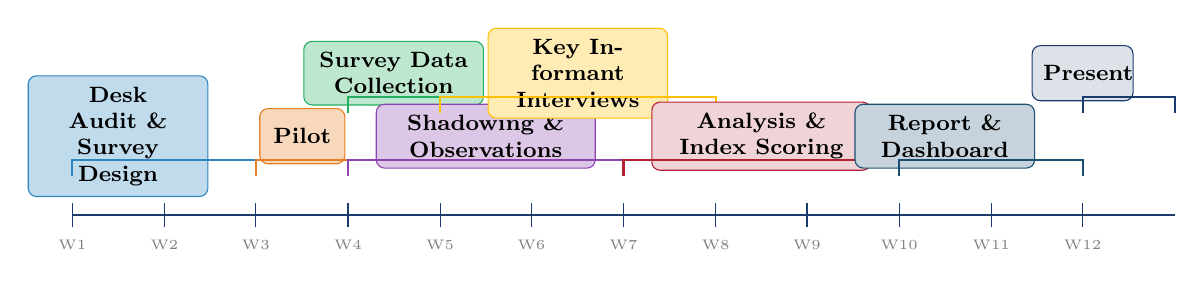
\begin{tikzpicture}[
    phase/.style={rectangle, rounded corners=3pt, minimum height=0.7cm, 
                  align=center, font=\footnotesize\bfseries, inner sep=4pt},
    wk/.style={font=\tiny, color=gray}
]
    % Timeline axis
    \draw[thick, govblue] (0,0) -- (14,0);
    \foreach \x/\w in {0/1, 1.17/2, 2.33/3, 3.5/4, 4.67/5, 5.83/6, 7/7, 8.17/8, 9.33/9, 10.5/10, 11.67/11, 12.83/12} {
        \draw[govblue] (\x, -0.15) -- (\x, 0.15);
        \node[wk, below] at (\x, -0.2) {W\w};
    }

    % Phase bars
    \node[phase, fill=accent2!30, draw=accent2, text width=2cm] at (0.58, 1.0) {Desk Audit \&\\Survey Design};
    \draw[accent2, thick] (0, 0.5) -- (0, 0.7) -- (2.33, 0.7) -- (2.33, 0.5);

    \node[phase, fill=accent4!30, draw=accent4, text width=0.8cm] at (2.92, 1.0) {Pilot};
    \draw[accent4, thick] (2.33, 0.5) -- (2.33, 0.7) -- (3.5, 0.7) -- (3.5, 0.5);

    \node[phase, fill=accent3!30, draw=accent3, text width=2cm] at (4.08, 1.8) {Survey Data\\Collection};
    \draw[accent3, thick] (3.5, 1.3) -- (3.5, 1.5) -- (5.83, 1.5) -- (5.83, 1.3);

    \node[phase, fill=accent5!30, draw=accent5, text width=2.5cm] at (5.25, 1.0) {Shadowing \&\\Observations};
    \draw[accent5, thick] (3.5, 0.5) -- (3.5, 0.7) -- (7, 0.7) -- (7, 0.5);

    \node[phase, fill=govgold!30, draw=govgold, text width=2cm] at (6.42, 1.8) {Key Informant\\Interviews};
    \draw[govgold, thick] (4.67, 1.3) -- (4.67, 1.5) -- (8.17, 1.5) -- (8.17, 1.3);

    \node[phase, fill=govred!20, draw=govred, text width=2.5cm] at (8.75, 1.0) {Analysis \&\\Index Scoring};
    \draw[govred, thick] (7, 0.5) -- (7, 0.7) -- (10.5, 0.7) -- (10.5, 0.5);

    \node[phase, fill=accent1!25, draw=accent1, text width=2cm] at (11.08, 1.0) {Report \&\\Dashboard};
    \draw[accent1, thick] (10.5, 0.5) -- (10.5, 0.7) -- (12.83, 0.7) -- (12.83, 0.5);

    \node[phase, fill=govblue!15, draw=govblue, text width=1cm] at (12.83, 1.8) {Present};
    \draw[govblue, thick] (12.83, 1.3) -- (12.83, 1.5) -- (14, 1.5) -- (14, 1.3);

\end{tikzpicture}
\caption{Phased 12-week research timeline. Overlapping phases reflect concurrent activities; e.g., shadowing occurs alongside survey administration, and interviews begin while survey collection continues.}
\label{fig:timeline}
\end{figure}

\begin{table}[H]
\centering
\caption{Detailed 12-Week Deliverables}
\label{tab:timeline_detail}
\begin{tabularx}{\textwidth}{@{}llX@{}}
\toprule
\textbf{Week} & \textbf{Phase} & \textbf{Deliverable} \\
\midrule
1--2 & Desk Audit + Design & Department profiles, questionnaire draft, sampling plan \\
3 & Pilot Test & Test survey on 5--10 employees; refine questions based on feedback \\
4--5 & Survey Collection & 120+ completed survey responses across 4 departments \\
4--6 & Shadowing & Field notes from 8 employee shadowing sessions \\
5--7 & Key Informant Interviews & 4--8 interview transcripts/summaries \\
8--9 & Analysis & GovTech Adoption Index scores; demographic cross-tabulations \\
10--11 & Report + Visualisation & Full \LaTeX\ report with charts; optional dashboard prototype \\
12 & Presentation & Final presentation to AIGGPA; policy brief submission \\
\bottomrule
\end{tabularx}
\end{table}

% =============================================================================
\section{Glossary (\hindi{शब्दावली})}

\begin{longtable}{@{}ll@{}}
\toprule
\textbf{Abbreviation} & \textbf{Full Form} \\
\midrule
\endfirsthead
\toprule
\textbf{Abbreviation} & \textbf{Full Form} \\
\midrule
\endhead
AEBAS & Aadhaar Enabled Biometric Attendance System \\
AIGGPA & Atal Bihari Vajpayee Institute of Good Governance \& Policy Analysis \\
APAR & Annual Performance Assessment Report \\
ARC & Administrative Reforms Commission \\
BPR & Business Process Re-engineering \\
CCA & Classification, Control and Appeal (Rules) \\
CGA & Controller General of Accounts \\
CPGRAMS & Centralised Public Grievance Redress \& Monitoring System \\
CSMOP & Central Secretariat Manual of Office Procedure \\
DARPG & Dept of Administrative Reforms \& Public Grievances \\
DBT & Direct Benefit Transfer \\
DoPT & Department of Personnel \& Training \\
DSC & Digital Signature Certificate \\
e-HRMS & Electronic Human Resource Management System \\
ESS & Employee Self-Service \\
GAD & General Administration Department \\
GeM & Government e-Marketplace \\
GEMS & Government Employees Management System \\
GMV & Gross Merchandise Value \\
GPI & Gender Parity Index \\
HMIS & Health Management Information System \\
iGOT & Integrated Government Online Training \\
ITCP & Integrated Treasuries Computerisation Project \\
KCM & Karmayogi Competency Model \\
KII & Key Informant Interview \\
LMS & Learning Management System \\
MAP\_IT & Madhya Pradesh Agency for Promotion of IT \\
MeitY & Ministry of Electronics \& Information Technology \\
MoCI & Ministry of Commerce \& Industry \\
MoF & Ministry of Finance \\
NeSDA & National e-Service Delivery Assessment \\
NEVA & National e-Vidhan Application \\
NIC & National Informatics Centre \\
PFMS & Public Financial Management System \\
RCMS & Revenue Court Case Management System \\
SeMT & State e-Governance Mission Team \\
SMART & Simple, Moral, Accountable, Responsive, Transparent \\
SPARROW & Smart Performance Appraisal Report Recording Online Window \\
SSO & Single Sign-On \\
SWAN & State Wide Area Network \\
TOE & Technology-Organization-Environment (Framework) \\
UDISE+ & Unified District Information System for Education Plus \\
\bottomrule
\end{longtable}

% =============================================================================
\section*{Data Integrity Declaration}

\begin{warningbox}[Zero-Hallucination Policy]
Every numerical figure, statistic, and factual claim in this document is sourced from verified secondary sources:

\begin{itemize}
  \item \textbf{Government of India:} PIB press releases, DARPG publications, DoPT Annual Reports, NIC Informatics journal, Digital India Corporation, CGA/PFMS documentation, GeM Annual Reports
  \item \textbf{Policy Documents:} 2nd Administrative Reforms Commission (11th Report), CSMOP 2019, CCS (CCA) Rules 1965, 7th Central Pay Commission
  \item \textbf{Institutional:} NITI Aayog, IndiaAI.gov.in, iGOT Karmayogi platform data, NeSDA Way Forward Reports
  \item \textbf{Academic/Research:} Emerald Insight, ResearchGate, IAPA, ADB reports, Wadhwani Foundation
  \item \textbf{Media (verified):} Economic Times, DD News, Tribune India, India Times (only for cross-referencing official data)
\end{itemize}

\textbf{Qualitative assessments} (e.g., ``High/Moderate/Low'' usage levels in Tables~\ref{tab:class1}--\ref{tab:class3}, and the qualitative scores in Figure~\ref{fig:class_comparison}) are derived from synthesis of the above sources and are clearly identified as analytical assessments, not raw data.

\textbf{No primary data} was collected for this report. For internship deliverables, this secondary research should be supplemented with primary data (surveys, interviews, field observations) collected at AIGGPA.
\end{warningbox}

\end{document}

